\documentclass[12pt,a4paper]{article}

\usepackage[left=2.50cm, right=2.50cm, top=2.50cm, bottom=2.50cm]{geometry}
\usepackage[onehalfspacing]{setspace}

\usepackage[utf8]{inputenc}
\usepackage[ngerman]{babel}
\usepackage[T1]{fontenc}
\usepackage[plainfootsepline, headsepline]{scrpage2}
\usepackage[autostyle=true,german=quotes]{csquotes}

\usepackage[bookmarks, colorlinks]{hyperref}
%hidelinks
%colorlinks
\usepackage{scrextend}
\usepackage[xindy, acronyms, nonumberlist]{glossaries}

\usepackage[square, numbers]{natbib}
\usepackage{pdfpages}

\usepackage{graphicx}
\usepackage{subfig}
\usepackage{wrapfig,lipsum}
\usepackage{xcolor}
\usepackage{verbatim}
\usepackage{listings}

\usepackage{eurosym}

% Befehl zur Realisierung von Inline-Code:
\newcommand{\code}[1]{\texttt{#1}}

\bibliographystyle{plainnat}
%\bibliographystyle{harvard}
\author{Manuel Bothner, Simon Lang}
\title{Studienarbeit}

\setheadsepline{1pt}[\color{black}]
\setlength{\headsep}{20 mm}

\makeglossaries
%abbreviations
\newacronym[longplural={Applications}]{app}{App}{Application}
\newacronym{tcp}{TCP}{Transmission Control Protocol}
\newacronym{json}{JSON}{JavaScript Object Notation}
\newacronym{mvvm}{MVVM}{Model View ViewModel}
\newacronym{uml}{UML}{UMnified Modeling Language}
\newacronym{cpu}{CPU}{Central Processing Unit}

%glossaries
\newglossaryentry{javascript}
{
	name=JavaScript,
	description={Skriptsprache zur Entwicklung dynamischer Internetseiten}
}
\newglossaryentry{typescript}
{
	name=TypeScript,
	description={Objektorientierte Programmiersprache für Webentwicklung}
}
\newglossaryentry{framework}
{
	name=Framework,
	description={Rahmen zur Programmierung mit verschiedenen Softwarekomponenten},
	plural=Frameworks
}
\newglossaryentry{java}
{
	name=Java,
	description={Objektorientierte Programmiersprache für plattformübergreifende Anwendungen}
}
\newglossaryentry{objectivc}
{
	name=Objective-C,
	description={Auf C basierte objektorientierte Programmiersprache}
}
\newglossaryentry{template}
{
	name=Template,
	description={Vorlage zur Implementierung}
}
\newglossaryentry{csharp}
{
	name=C\#,
	description={Objektorientierte Programmiersprache mit dem Schwerpunkt auf Typsicherheit}
}
\newglossaryentry{lejos}
{
	name=leJos,
	description={Java System zur Programmierung von LEGO Mindstorm}
}
\newglossaryentry{ev3}
{
	name=EV3,
	description={Kleinroboter der LEGO Mindstorm Serie}
}
\newglossaryentry{eclipse}
{
	name=Eclipse,
	description={Programmierumgebung für diverse Programmiersprachen und Frameworks}
}
\newglossaryentry{javafx}
{
	name=JavaFX,
	description={Framework zur Erstellung von Java Anwendungen}
}
\newglossaryentry{sqlite}
{
	name=SQLite,
	description={Bibliothek zur Erstellung einer lokalen relationalen Datenbank}
}

%dual entry
\newglossaryentry{gls-api} {
	name={Application Programming Interface},
	description={Programmierschnittstelle, die die Anbindung von Software ermöglicht},
}
\newacronym[see={[Glossary:]{gls-api}}]{api}{API}{Application Programming Interface\glsadd{gls-api}}
\newglossaryentry{gls-html}
{
	name=Hypertext Markup Language,
	description={Basiert auf XML und bestimmt den Aufbau einer Internetseite},
}
\newacronym[see={[Glossary:]{gls-html}}]{html}{HTML}{Hypertext Markup Language\glsadd{html}}
\newglossaryentry{gls-css}
{
	name=Cascading Style Sheets,
	description={Bestimmt das Design einer Internetseite}
}
\newacronym[see={[Glossary:]{gls-css}}]{css}{CSS}{Cascading Style Sheets\glsadd{css}}
\newglossaryentry{gls-xml}
{
	name=Extensible Markup Language,
	description={Ein auf Text basiertes Format zum Austausch von Informationen und Daten}
}
\newacronym[see={[Glossary:]{gls-xml}}]{xml}{XML}{Extensible Markup Language\glsadd{xml}}
\newglossaryentry{gls-ui}
{
	name=User Interface,
	description={Eine Nutzerschnittstelle, zur Interaktionen mit der Anwendung}
}
\newacronym[see={[Glossary:]{gls-ui}}]{ui}{UI}{User Interface\glsadd{ui}}
\newglossaryentry{gls-gui}
{
	name=Graphical User Interface,
	description={Eine grafische Nutzerschnittstelle, zur Interaktionen mit der Anwendung}
}
\newacronym[see={[Glossary:]{gls-gui}}]{gui}{GUI}{Graphical User Interface\glsadd{gui}}
\newglossaryentry{gls-aot}
{
	name=Ahead of Time,
	description={Übersetzt Programmcode vor der Ausführung in Maschinencode}
}
\newacronym[see={[Glossary:]{gls-aot}}]{aot}{AOT}{Ahead of Time\glsadd{aot}}
\newglossaryentry{gls-arm}
{
	name=Acorn RISC Machines,
	description={Mikroprozessordesign}
}
\newacronym[see={[Glossary:]{gls-arm}}]{arm}{ARM}{Acorn RISC Machines\glsadd{arm}}
\newglossaryentry{gls-il}
{
	name=Intermediate Language,
	description={Intermediate Language ist eine objektorientierte Assemblersprache}
}
\newacronym[see={[Glossary:]{gls-il}}]{il}{IL}{Intermediate Language\glsadd{il}}
\newglossaryentry{gls-jit}
{
	name=Just-in-Time,
	description={Der entsprechende Quellcode wird zur Laufzeit übersetzt}
}
\newacronym[see={[Glossary:]{gls-jit}}]{jit}{JIT}{Just-in-Time\glsadd{jit}}
\newglossaryentry{gls-dll}
{
	name=Dynamic Linked Library,
	description={Dynamische Bibliothek, die zur Laufzeit dem Programmcode hinzugefügt wird},
	plural=DLLs
}
\newacronym[see={[Glossary:]{gls-dll}}]{dll}{DLL}{Dynamic Linked Library\glsadd{dll}}
\newglossaryentry{gls-cli}
{
	name=Common Language Infrastructure,
	description={Spezifikation zur sprach- und plattformneutralen Entwicklung von Anwendungen}
}
\newacronym[see={[Glossary:]{gls-cli}}]{cli}{CLI}{Common Language Infrastructure\glsadd{cli}}
\newglossaryentry{gls-clr}
{
	name=Common Language Runtime,
	description={Laufzeitumgebung zur Ausführung von .NET Anwendungen}
}
\newacronym[see={[Glossary:]{gls-clr}}]{clr}{CLR}{Common Language Runtime\glsadd{clr}}
%###########################################################################################################################################
%### TERMINILOGIE FESTLEGUNG ###############################################################################################################
%###########################################################################################################################################

%### Beschreibung ###################################################################################%
%# Dieses Dokument dient zur Festlegung der Terminoligie. Hier können Begriffe die bestimmte Kompo- #%
%# nenten, Systeme oder Sachverhalte beschreiben festgelegt und Variablen zugeordnet werden. Die    #%
%# Verwendung dieser Variablen in der Ausarbeitung soll sicherstellen das für eine Komponente, ein  #%
%# System oder Sachverhalt immer der selbe Begriff verwendet wird.                                  #%
%#                                                                                                  #%
%# Beispiel:                                                                                        #%
%# Für das (Netzwerk-)Konfigurations-Management kann es leicht passieren das Begriffe (bzw. unter-  #%
%# schiedliche Schreibweisen) wie:                                                                  #%
%# - Netzwerk-Konfigurationsmanagement                                                              #%
%# - Netzwerkkonfigurationsmanagement                                                               #%
%# - Netzwerk-Konfigurations-Management                                                             #%
%# oder auch nur                                                                                    #%        
%# - Konfigurations-Management                                                                      #%
%# - Konfigurationsmanagement                                                                       #%
%# Verwendet werden obwohl immer das selbe (der selbe Managementbereich) gemeint ist. Diese Inkon-  #%
%# sistenz führt zu Verwirrung des Lesers, dem nicht klar ist ob ein und das selbe oder etwas an-   #%
%# deres geweint ist. Darüber hinaus ist es kein guter Stiel.                                       #%
%#                                                                                                  #%
%# Aus diesem Grund wird der Begriff der eine Komponente, ein System etc. beschreibt einmal ein-    #%
%# deutig festgelegt und dann ausschließlich dieser verwendet.                                      #%
%#                                                                                                  #%
%# Verwendung:                                                                                      #%
%# Eine variable die ein Begriff darstellt wir wie folgt definiert:                                 #%
%# \newcommand{\terKM}{Konfigurations-Management}                                                   #%
%# Im Text verwendet wird die Variable (der Begriff) mit:                                           #%
%# \terKM{}                                                                                         #%
%# Dazu muss dieses Dokument einmal via %###########################################################################################################################################
%### TERMINILOGIE FESTLEGUNG ###############################################################################################################
%###########################################################################################################################################

%### Beschreibung ###################################################################################%
%# Dieses Dokument dient zur Festlegung der Terminoligie. Hier können Begriffe die bestimmte Kompo- #%
%# nenten, Systeme oder Sachverhalte beschreiben festgelegt und Variablen zugeordnet werden. Die    #%
%# Verwendung dieser Variablen in der Ausarbeitung soll sicherstellen das für eine Komponente, ein  #%
%# System oder Sachverhalt immer der selbe Begriff verwendet wird.                                  #%
%#                                                                                                  #%
%# Beispiel:                                                                                        #%
%# Für das (Netzwerk-)Konfigurations-Management kann es leicht passieren das Begriffe (bzw. unter-  #%
%# schiedliche Schreibweisen) wie:                                                                  #%
%# - Netzwerk-Konfigurationsmanagement                                                              #%
%# - Netzwerkkonfigurationsmanagement                                                               #%
%# - Netzwerk-Konfigurations-Management                                                             #%
%# oder auch nur                                                                                    #%        
%# - Konfigurations-Management                                                                      #%
%# - Konfigurationsmanagement                                                                       #%
%# Verwendet werden obwohl immer das selbe (der selbe Managementbereich) gemeint ist. Diese Inkon-  #%
%# sistenz führt zu Verwirrung des Lesers, dem nicht klar ist ob ein und das selbe oder etwas an-   #%
%# deres geweint ist. Darüber hinaus ist es kein guter Stiel.                                       #%
%#                                                                                                  #%
%# Aus diesem Grund wird der Begriff der eine Komponente, ein System etc. beschreibt einmal ein-    #%
%# deutig festgelegt und dann ausschließlich dieser verwendet.                                      #%
%#                                                                                                  #%
%# Verwendung:                                                                                      #%
%# Eine variable die ein Begriff darstellt wir wie folgt definiert:                                 #%
%# \newcommand{\terKM}{Konfigurations-Management}                                                   #%
%# Im Text verwendet wird die Variable (der Begriff) mit:                                           #%
%# \terKM{}                                                                                         #%
%# Dazu muss dieses Dokument einmal via %###########################################################################################################################################
%### TERMINILOGIE FESTLEGUNG ###############################################################################################################
%###########################################################################################################################################

%### Beschreibung ###################################################################################%
%# Dieses Dokument dient zur Festlegung der Terminoligie. Hier können Begriffe die bestimmte Kompo- #%
%# nenten, Systeme oder Sachverhalte beschreiben festgelegt und Variablen zugeordnet werden. Die    #%
%# Verwendung dieser Variablen in der Ausarbeitung soll sicherstellen das für eine Komponente, ein  #%
%# System oder Sachverhalt immer der selbe Begriff verwendet wird.                                  #%
%#                                                                                                  #%
%# Beispiel:                                                                                        #%
%# Für das (Netzwerk-)Konfigurations-Management kann es leicht passieren das Begriffe (bzw. unter-  #%
%# schiedliche Schreibweisen) wie:                                                                  #%
%# - Netzwerk-Konfigurationsmanagement                                                              #%
%# - Netzwerkkonfigurationsmanagement                                                               #%
%# - Netzwerk-Konfigurations-Management                                                             #%
%# oder auch nur                                                                                    #%        
%# - Konfigurations-Management                                                                      #%
%# - Konfigurationsmanagement                                                                       #%
%# Verwendet werden obwohl immer das selbe (der selbe Managementbereich) gemeint ist. Diese Inkon-  #%
%# sistenz führt zu Verwirrung des Lesers, dem nicht klar ist ob ein und das selbe oder etwas an-   #%
%# deres geweint ist. Darüber hinaus ist es kein guter Stiel.                                       #%
%#                                                                                                  #%
%# Aus diesem Grund wird der Begriff der eine Komponente, ein System etc. beschreibt einmal ein-    #%
%# deutig festgelegt und dann ausschließlich dieser verwendet.                                      #%
%#                                                                                                  #%
%# Verwendung:                                                                                      #%
%# Eine variable die ein Begriff darstellt wir wie folgt definiert:                                 #%
%# \newcommand{\terKM}{Konfigurations-Management}                                                   #%
%# Im Text verwendet wird die Variable (der Begriff) mit:                                           #%
%# \terKM{}                                                                                         #%
%# Dazu muss dieses Dokument einmal via \input{PATH\terminology} in das Textdokument eingebunden    #%
%# werden.                                                                                          #%
%# Manchmal empielt es sich die Trennstellen des Wortes mit anzugeben z.B.:                         #%
%# \newcommand{\KM}{Konfigu\-rations-Manage\-ment}                                                  #%
%####################################################################################################%

%### Variablen/Begriffs Deklaration ########################################################################################################

%Beispiele:
\newcommand{\LE}{LEGO}
\newcommand{\LM}{LEGO MINDSTORMS}


%###########################################################################################################################################
%### EOF ###################################################################################################################################
%########################################################################################################################################### in das Textdokument eingebunden    #%
%# werden.                                                                                          #%
%# Manchmal empielt es sich die Trennstellen des Wortes mit anzugeben z.B.:                         #%
%# \newcommand{\KM}{Konfigu\-rations-Manage\-ment}                                                  #%
%####################################################################################################%

%### Variablen/Begriffs Deklaration ########################################################################################################

%Beispiele:
\newcommand{\LE}{LEGO}
\newcommand{\LM}{LEGO MINDSTORMS}


%###########################################################################################################################################
%### EOF ###################################################################################################################################
%########################################################################################################################################### in das Textdokument eingebunden    #%
%# werden.                                                                                          #%
%# Manchmal empielt es sich die Trennstellen des Wortes mit anzugeben z.B.:                         #%
%# \newcommand{\KM}{Konfigu\-rations-Manage\-ment}                                                  #%
%####################################################################################################%

%### Variablen/Begriffs Deklaration ########################################################################################################

%Beispiele:
\newcommand{\LE}{LEGO}
\newcommand{\LM}{LEGO MINDSTORMS}


%###########################################################################################################################################
%### EOF ###################################################################################################################################
%###########################################################################################################################################
%###########################################################################################################################################
%### FARB-FESTLEGUNG ###############################################################################################################
%###########################################################################################################################################

% Farben für Text-Zustand:
\definecolor{template}{HTML}{EC008C}
\definecolor{process}{HTML}{C50D0D}
\definecolor{finishing}{HTML}{FB5801}
\definecolor{finished}{HTML}{FFC100}
\definecolor{corrected}{HTML}{3EC605}


%###########################################################################################################################################
%### EOF ###################################################################################################################################
%###########################################################################################################################################
\glsaddall

\begin{document}
	
	\pagestyle{scrheadings}
\clearscrheadfoot
\ihead{
\includegraphics[scale=0.8]{images/icon_dhbw.jpg}}
\begin{verbatim}
\end{verbatim}
\begin{center}
	\large{\textbf{Konzeption und Implementierung eines Sachwarmverhaltens von mobilen Kleinrobotern anhand eines Verfolgungsszenarios}}
\end{center}
\begin{verbatim}

\end{verbatim}
\begin{center}
	\large{STUDIENARBEIT}
\end{center}
\begin{verbatim}

\end{verbatim}
\begin{center}
	für die Prüfung zum\\
	\medskip
	Bachelor of Science\\
	\medskip
	des Studiengangs Informatik\\
	Studienrichtung Angewandte Informatik\\
	\medskip
	an der\\
	\medskip
	Dualen Hochschule Baden-Württemberg Karlsruhe\\
\end{center}
\begin{verbatim}
\end{verbatim}
\begin{center}
	\today
\end{center}
\begin{verbatim}





\end{verbatim}	
\begin{flushleft}
	\begin{tabular}{p{4cm} p{6cm} p{6cm}}
		Name & Manuel Bothner & Simon Lang\\
		Matrikelnummer & 8359139 & 6794837\\
		Kurs & TINF14B2 & TINF14B2\\
		Ausbildungsfirma & 1\&1 Internet SE & ifm ecomatic GmbH\\
		& Brauerstr. 48 & Im Heidach 18\\
		& 76135 Karlsruhe & 88079 Kressbronn am Bodensee\\
		Betreuer & Prof. Hans-Jörg Haubner & \\
	\end{tabular}
\end{flushleft}
		\pagestyle{scrheadings}
	\clearscrheadfoot
	\ohead{
\includegraphics[scale=0.6]{images/icon_dhbw.jpg}}
	
	\section*{Erklärung}
	
	(gemäß §5(3) der „Studien- und Prüfungsordnung DHBW Technik“ vom 29. 9. 2015)\\
	Ich versichere hiermit, dass ich meine Projektarbeit mit dem Thema: \enquote{Konzeption und Implementierung eines Sachwarmverhaltens von mobilen Kleinrobotern anhand eines Verfolgungsszenarios} selbstständig verfasst und keine anderen als die angegebenen Quellen und Hilfsmittel benutzt habe. Ich versichere zudem, dass die eingereichte elektronische Fassung mit der gedruckten Fassung übereinstimmt.
	\begin{verbatim}
	\end{verbatim}
	\noindent\rule{\textwidth}{1pt}
	\noindent Ort, Datum\hfill\hfill Unterschrift
	\section*{Abstract}

\newpage
\section*{Zusammenfassung}
	\tableofcontents
	\setcounter{page}{1}
\ofoot{\pagemark}

\section{Einleitung}

Heutzutage werden viele Arbeitsschritte im Agrar-, Industrie- und Dienstleistungssektor von Computern und Roboter verrichtet, da diese eine effizientere Arbeit leisten und weniger Kosten als Menschen verursachen. Diese Technologien erfuhren in den letzten Jahren einen immer stärkeren Wandel durch laufende technische Innovationen, die deren Arbeitsablauf verbessern und somit produktiver gestalten.
Eine dieser Technologien stellt das theoretische Konzept eines Schwarmverhaltens dar, welches Unternehmen zur Kooperation verschiedener Computer und Roboter einsetzen. Dies ermöglicht die gegenseitige Unterstützung der Komponenten und somit einen geteilten Arbeitsablauf, um die jeweiligen Stärken zu nutzen. Diese Verhaltensstrukturen stammen meist aus der Tierwelt, wie am Beispiel von Fischschwärmen, Ameisen oder Bienen, wobei jedes Individuum des Schwarms seine Aufgeben für das Überleben des Schwarms erfüllt.\\
In diesem Projekt werden die grundlegenden Verhaltensstrukturen von in Schwärmen lebenden Tieren zur Umsetzung eines Verfolgungsszenarios, wie am Beispiel eines autonom fahrenden Autos, aufgegriffen. Dabei werden feste Regeln anhand von Benutzerszenarios definiert, auf welche der Roboterschwarm entsprechend der Nutzerhandlungen reagiert. Dies wird durch ein zentrales Kommunikationssystem umgesetzt, an welches alle teilnehmenden Komponenten angeschlossen sind.\\
Die Einsatzgebiete dieses Projektes sind dabei entsprechend groß und kann überall eingesetzt werden, wo technische Komponenten für ein gemeinsames Produkt zusammenarbeiten müssen. Beispiele hierfür ist die Optimierung von Produktionsanlagen, oder Verkehrsführungen in Form von autonom fahrenden Autos.

\newpage
\subsection{Ausgangslage}

Die Ausgangslage des Projektes stellen verschiedene Computer und Roboter ohne intelligentes Kommunikationssystem dar, welche einen Mehrwert durch eine Dienstleistung oder die Bearbeitung eines Produktes erwirtschaften. In diesem Projekt wird dies durch den Einsatz von LEGO Mindstorm EV3 Roboter dargestellt, welche mittels Struktur orientierter Programmierung verwendet werden können. Diese verfügen über verschiedene Schnittstellen sowie Sensorik, um mit ihrer Umwelt interagieren zu können und stellen damit die Basis eines Schwarmes dar.

\begin{itemize}
	\item LEGO Mindstorm EV3
	\item LEGO Mindstorm Sensorik
	\item Kabellose Netzwerkschnittstelle
\end{itemize}

\subsection{Zielsetzung}

Das Ziel dieser Studienarbeit stellt die Implementierung eines Schwarmverhaltens mit dem Fokus auf ein Verfolgungsszenario zwischen Kleinrobotern dar. Dabei soll ein zentrales Kommunikationssystem aufgebaut werden, auf dessen Grundlage die Komponenten miteinander interagieren. Die Roboter enthalten hierbei Grundfunktionen, die über Kommandos des Kommunikationssystems angesprochen werden, um die definierten Benutzerszenarios auszuführen und den Roboter zu bewegen.

\begin{itemize}
	\item Zentrales Kommunikationssystem
	\item Grundlegende Steuerungsfunktionen
	\item Abbildung von Schwarmverhalten
	\item Darstellung der aktuellen Daten
\end{itemize}

\begin{comment}
	\subsection{Erwartetes Ergebnis}
	
	Erwartet wird ein Ergebnis, indem der Nutzer des Systems über eine mobile App mithilfe einer zentralen STeuereinheit einen beliebigen Kontext für ein ausgewähltes Schwarmverhalten starten kann. Dabei soll eine abstrakte IMplementierung beachtet werden, indem verschiedene RObotertypen und Szenarien für Schwarmverhalten dargestellt sind, um wenn erwünscht ein komplexes Szanrio mit unterschiedlichen RObotern zu starten um definierte AUfgaben zu lösen. Dabei ist vor allem die Implementierung der Grundsteuerung mitsammt der Kommunikation des Systems entscheident.
\end{comment}
	\section{Technische Grundlagen}
\subsection{Robotik} % Manuel ca. 8
% Farbe die angibt welchen Status der folgende Abschnitt hat:
\color{finishing}
% Eigentlicher Text:
Die Robotik beschäftigt sich mit dem Entwurf, der Konstruktion sowie der Programmierung, Steuerung und dem Betrieb 
von Robotern \newline [http://wirtschaftslexikon.gabler.de/Definition/robotik.html]. Dabei umfasst die Robotik eine Vielzahl 
von Fachgebieten wie der Elektrotechnik, dem Maschienenbau, der Informatik sowie der Biologie und der Medizin.
\subsubsection{Roboter}
% Farbe die angibt welchen Status der folgende Abschnitt hat:
\color{finishing}
% Eigentlicher Text:
Was im Kontext der Robotik unter einem Roboter zu verstehen ist, ist gar nicht so einfach darzulegen, da es in Tat keine allgemein anerkannte Definition dieses Begriffs gibt, die seiner üblichen Verwendung entspricht [Mobile Roboter - 2].
\newline
Auch ohne eine vollkommen allgemeingültige und präzise Beschreibung eines Roboters zu sein, soll hier die VDI-Richtline 2860 einen Eindruck darüber vermitteln, was in der Robotik mit Roboter gemeint ist. \newline
Die VDI-Richtline 2860 von 1990 definiert einen Roboter wie folgt:
\vspace{2mm}
\newline
>>\textit{Ein Roboter ist ein frei und wieder programmierbarer, multifunktio-
naler Manipulator mit mindestens drei unabhängigen Achsen, um Ma-
terialien, Teile, Werkzeuge oder spezielle Geräte auf programmierten,
variablen Bahnen zu bewegen zur Erfüllung der verschiedensten Auf-
gaben.}<<
\vspace{2mm}
\newline
Auch wenn diese Definition einige grundlegenden Eigenschaften eines Roboters darlegt, beschreibt diese Definition den Begriff des Roboters im industriellen Kontext und trifft hauptsächlich auf stationäre Industrieroboter zu, wie sie in der Automobilfertigung beispielsweise als Schweiß- oder Lackierroboter  verwendet werden. Die genannten programmierten Bahnen sind dort möglich, weil die Arbeitsprozess und die Umgebung auf den Roboter zugeschnitten und vollständig bekannt sind [MR 2]. \newline
Im Gegensatz dazu trifft dieser Aspekt auf mobile Roboter nicht zu. Mobile Roboter wie beispielsweise Service-Roboter bewegen sich in einer unsttrukturierten und dynamischen Umgebung.
\subsubsection{Mobile Roboter}
% Farbe die angibt welchen Status der folgende Abschnitt hat:
\color{process}
% Eigentlicher Text:
Mobile Roboter sind in ihrer Position variable, bewegen sich selbständig von
Ort zu Ort und interagieren mit ihrer Umgebung. Diese macht es notwendig das die Roboter ihre Umgebung erfassen und wahrnehmen können um auf Veränderungen wie bespielsweise Hindernisse reagieren zu können. \newline
...
\newline
Zu den Vertretern mobiler Roboter zählen zum Beispiel Service-Roboter, Erkundungsroboter und Humanoide Roboter. Im Folgenden sind einige Beispiele
für mobile Roboter dargelegt:
\begin{itemize}
	\item{\textbf{Shakey:}} Shakey war ein mobiler Roboter der von 1966 bis 1972 an der am Stanford Research Institute entwickelt wurde. Seine Entwicklung leistete wichtige Beiträge für die Robotik sowie in der KI-Forschung im Bereich der Handlungsplanung und dem selbständigen Lernen [MR 5f].
	%##################################################
	\item{\textbf{Spirit \& Opportunity:}} Spirit \& Opportunity sind zwei baugleiche Roboter die im Jahr 2003 von der NASA zum Mars geschickt wurden um den Himmelskörper zu erkunden. Die beiden Erkundungsroboter sind Radfahrzeuge mit flexiblem Fahrgestell, verfügen über eine Panoramakamera sowie Sensoren zur Untersuchung des Erdbodens und Gesteins. Obwohl die Roboter in Bezug auf ihrer gundsätzlichen Aktionen von der Erde aus ferngesteuert werden, ist eine autonome Steuerung welche auf kurzfristige, unerwartet Ereignisse wie das Wegrutschen von Rädern reagiert aufgrund der langen Signallaufzeiten unverzichtbar. Die Roboter waren für eine
	Lebensdauer von 90 Marstagen ausgelegt, übertrafen diese aber bei weitem (mehr als das 30fache) [MR 8f]
	%##################################################
	\item{\textbf{Stanley:}} Stanley ist ein vollständig autonomer Roboter der 2005 am Grand Challenge Wetbewerb teilnahm und diesem gewann. Bei diesem Wettbewerb mussten Fahrzeuge ohne Eingriff von Menschen eine festgelegte, jedoch nicht markierte Strecke von rund 213 km von einem definierten Start- zu einem definierten Zielpunkt zurücklegen. Die Strecke führte durch 
	die Mojave-Wüste in den USA. Bei Stanley handelt es sich um einen modifizierter VW Touareg, dem Sensoren zur Umgebungswahrnehmung und Bordrechner zur Bearbeitung des Kontrollprogramms eingebaut wurden. Stanleys wichtigste Umgebungssensoren waren mehrere Laserscanner und eine Kamera.Stanley meisterte die 213 km lange Strecke welche unter anderem durch felsige
	oder sandige Bereiche sowie durch Wasserläufe führte in knapp unter 7 Stunden.
	%##################################################
	\item{\textbf{Tribot}} D
\end{itemize}
Die Beispiele zeigen wie vielfältig ...
Neben der Forschung -> Marktpotenzial erwähnen
\subsubsection{Sensorik}
% Farbe die angibt welchen Status der folgende Abschnitt hat:
\color{process}
% Eigentlicher Text:
Um mit der Umgebung interagieren zu können müssen mobile Roboter diese wahrnehmen, dazu dienen Sensoren. Sensoren ermöglichen es dem Roboter Informationen über seine Umwelt und über seinen Zustand zu sammeln.
Sensoren lassen sich hinsichtliche ihrer Arbeitsweise und ... wie folgt klassifizieren:
\begin{itemize}
	\item{\textbf{Propriozeptive Sensoren}} -- Diese Art der Sensoren bestimmen eine Messgröße des Roboters selbst und haben keine \glqq{}Kontakt\grqq{} zur Umwelt z.B Bestimmung der Lage Aufgrund eines Neigungssensors.
	\item{\textbf{Exterozeptive Sensoren}} -- Im Gegensatz zu den propriozeptive Sensoren gewinnen diese Sensoren Informationen aus Messgrößen der Umwelt beispielsweise die Bestimmung der Orientierung in Bezug auf die Umwelt.
	\item{\textbf{Aktive Sensoren}} -- Aktive Sensoren senden aktive Energie in ihre Umwellt aus und Erfassen anschließend die zurückkehrenden Signale wie dies beispielsweiße ein Ultraschallsensor tut.
	\item{\textbf{Passive Sensoren}} -- Diese Sensoren senden nicht aktiv aus sondern erfassen ausschließlich die von Natur aus vorhandenen Signale wie z.B. das einfallende Licht durch eine Kamera.
\end{itemize}
Die folgenden Tabelle zeigt beispielhaft die Einordnung einiger Sensoren:
\begin{table}[ht]
	\begin{tabular}{|p{4,5cm}|p{4,0cm}|p{4,0cm}|} \hline
		     	                & Aktive Sensoren      & Passive Sensoren   \\ \hline
		Propriozeptive Sensoren & 
			(Inkrementalgeber (Photoelektrische Abtastung)) & 
			Inkrementalgeber, \newline Neigungssensor, \newline Gyroskop   \\ \hline
		Exterozeptive Sensoren  & 
			Ultraschallsensor,  \newline Laserscanner, \newline Infrarotsensor, \newline Radar    & 
			Kontaktsensor, \newline Kompass, \newline Kamera, \newline GPS      \\ \hline 
	\end{tabular}
	\centering
	\caption[Einordnung von Sensoren]{Einordnung von Sensoren}
\end{table}
\subsubsection{Sensordatenverarbeitung}
\subsubsection{Antriebsarten}
\subsection{\LM}
% Farbe die angibt welchen Status der folgende Abschnitt hat:
\color{finishing}
% Eigentlicher Text:
\LM{} ist eine seit 1988 existierende Produktserie des Spielwarenherstellers \LE{} \cite[vgl.][21]{Scholz.DasEV3}. 
\LM{} ermöglicht das Bauen, Programmieren und Steuern verschiedener \LE{} Roboter. Dies Roboter bestehen dabei aus
gängigen \LE{} Teilen die auch in anderen \LE{}-Produkten Verwendung finden, sowie speziellen \LE{}-Komponenten 
wie einer zentralen Steuereinheit, Motoren und Sensoren.
%-------------------------------------------------------------------------------------------------------------------------------------------
%### Subsektion über XXX ###################################################################################################################
%-------------------------------------------------------------------------------------------------------------------------------------------
\subsubsection{Das EV3-System}
% Farbe die angibt welchen Status der folgende Abschnitt hat:
\color{finishing}
% Eigentlicher Text:
Der 2013 erschienene EV3 ist das dritte System der \LM{} Reihe. Die Bezeichnung setzt sich aus EV für Evolution 
und 3 für die 3 Stufe der \LM{}-Serie zusammen \cite[vgl.][Seite 21]{Scholz.DasEV3}. \\
Im Vergleich zu den Vorgängersystemen verfügt das EV3-System über eine modernere und leistungsfähigere Steuereinheit und auch die anderen elektronischen Komponenten des System wurden an den heutigen Stand der Technik 
angepasst \cite[vgl.][Seite 22]{Scholz.DasEV3}.
\medskip
\newline
Die folgende Abbildung X.X zeigt einige der zentralen Komponeten des EV3-Systems, wie die Steuereinheit (EV3-Stein), Motoren und vier Sensoren.
\begin{figure}[ht]
	\centering
	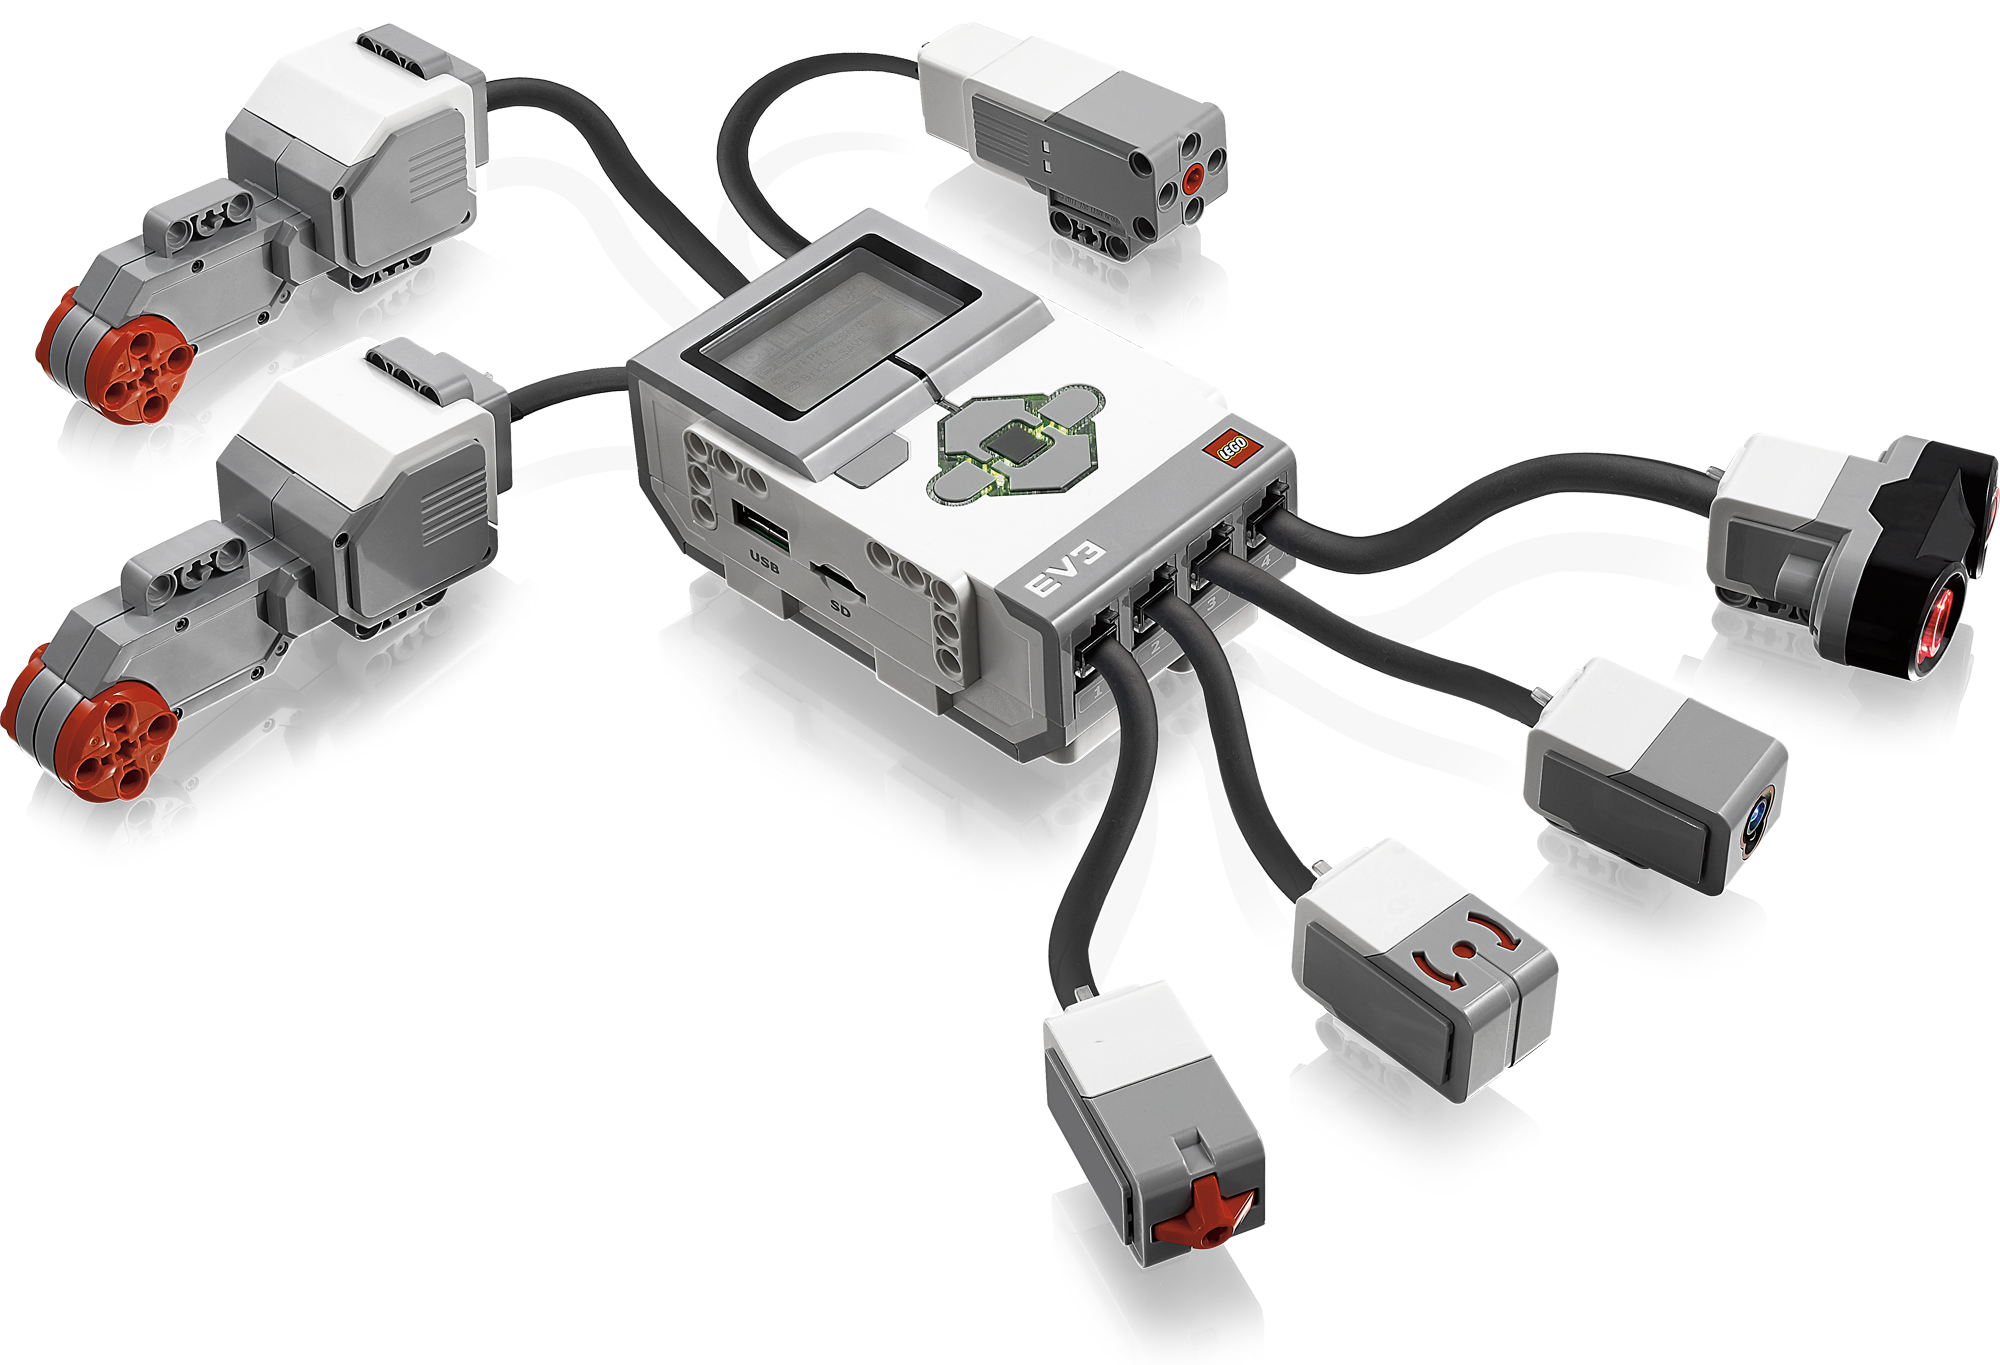
\includegraphics[width=0.90\textwidth]{images/technische_grundlagen/EV3-Overview.png}
	\caption[Zentrale Komponenten des EV3-Systems]{Zentrale Komponenten des EV3-Systems}
	\label{fig:<Sprungmakre>}
\end{figure}
\newline
Neben den elektronischen Komponeten gehören auch nicht elektronische Teile wie Verbindungsstücke, Balken und Zahnräder 
wie sie aus gängigen \LE{} Produkten bekannt sind, zum EV3-System. Sie bilden die strukturelle und meschanische Grundlage 
der Roboter.
\medskip
\newline
Im Folgenden wird auf die elektronischen Komponenten des EV3-Systems näher eingegangen.
dieses Projekt eine deutlich größere Relevanzu aufweisen.
\subsubsection{Der EV3-Stein (Steuereinheit)}
% Farbe die angibt welchen Status der folgende Abschnitt hat:
\color{finishing}
% Eigentlicher Text:
Die zentrale Komponenten und das Gehirn des LEGO MINDSTORMS EV3-Systems ist die zentrale Steuereinheit kurz (EV3-)Stein oder auch Brick genannt. Bei ihm handelt
es sich um eine Computer welcher selbständig Programme ausführen kann. Dazu verfügt der EV3-Stein über 
ein Linux Betriebssystem und eine spezielle Firmware, die wie die auszuführenden Programme auf einem Flash-Speicher liegen \cite[vgl.][21]{Scholz.DasEV3}. \\
Zur Kommunikation mit dem PC verfügt der EV3-Stein über eine USB- sowie Bluetooth-Schnittstelle. Neben der 
Kommunikation zu einem Computer kann die USB-Schnittstelle auch für den Zusammenschluss mit einem weiteren EV3-Stein (genannt Daisy Chain) 
genutzt werden \cite[vgl.][Seite 21]{Scholz.DasEV3}.  \\
Für den Anschluss von Motoren und Sensoren verfügt der EV3-Stein über 8 Ports, an welche die anderen System-Komponenten müber Kabel mit RJ12-Steckern angeschlossen werden. 4 der Ports dienen für den Anschluss von
Motoren, die restlichen 4 Ports für die Abfrage von Sensorwerte \cite[vgl.][21]{Scholz.DasEV3}.  \\
Der EV3-Stein besitzt an der Vorderseite ein LCD-Display zur Anzeige von Texten und Grafiken sowie  
6 Knöpfe für die Bedienung durch den Benutzer. Display und Knöpfe dienen zur Bedienung der Firmware sowie zur Tätigung von Einstellungen, können aber ebenso durch Programmen angesprochen und ausgewertet werden
Start
Mein Kanal
Trends
Abos
BIBLIOTHEK
\cite[vgl.][21]{Scholz.DasEV3}. 
\smallskip
\newline
Die folgende Auflistung zeigt einige Leistungsmerkmale des EV3-Steins \citep[vgl.][Seite 23 f., Seite 32]{Scholz.DasEV3, Schobel.RobertaEV3Programmieren}.
\begin{itemize}
	\item{Prozessor:} ARM9 32Bit, 300 MHz, 16 MB Flash 64MB RAM
	\item{Betriebssystem:} Linux
	\item{Sensoranschlüsse:} 4x, Analog / Digital bis zu 460,8 Kbit/s
	\item{USB-Schnittstellen:} 2x, für Kommunikation zum PC, Daisy Chain, WiFi-Stick, USB-Speichermedium
	\item{SD-Karten-Lesegerät:} 1x, für MicroSD-Karte bis 32 GB
	\item{User-Interface:} 6 Knöpfe inkl. Beleuchtung
	\item{Display:} LCD Matrix, monochrom, 178 x 128 Pixel
	\item{Kommunikation:} Bluetooth v2.1, USB 2.0 (Kommunikation zum PC), USB 1.1 (Daisy Chain)
\end{itemize}
\subsubsection{Motoren}
% Farbe die angibt welchen Status der folgende Abschnitt hat:
\color{finishing}
% Eigentlicher Text:
Das EV3-System verfügt über zwei unterschiedliche Motoren, einen großen Motor und einen mittleren Motor. 
Bei beiden handelt es sich um Servormotoren mit integriertem Rotationssensor, welche von außen angesteuert und abgefragt werden können \cite[vgl.][92]{Schobel.RobertaEV3Programmieren}. Die Motoren lassen sich sehr exakt steuern und ermöglichen so einen synchronen Betrieb mehrerer Motoren \cite[vgl.][Seite 29 f.]{Scholz.DasEV3}.
\smallskip
\newline
Die folgende Tabelle zeigt die wichtigsten Eigenschaften der beiden Motoren.
\begin{table}[ht]
	\begin{tabular}{|p{4,5cm}|p{4,0cm}|p{4,0cm}|} \hline
		Eigenschaft / Motortyp		                & Großer Motor         & Mittlerer Motor    \\ \hline
		Winkelgenauigkeit       & 1 $^\circ$           & 1 $^\circ$         \\ \hline
		Umdrehungen    			& 160 bis 170 U/min    & 240 bis 250 U/min  \\ \hline 
		Drehmoment Rotation		& 20 Ncm               & 8 Ncm    			\\ \hline  
		Drehmoment Stillstand 	& 40 Ncm               & 12 Ncm    			\\ \hline  
		Gewicht    				& 76g                  & 36g   		 		\\ \hline
	\end{tabular}
	\centering
	\caption[Eigenschaften der EV3-Motortypen]{Eigenschaften der EV3-Motoren}
\end{table}
\subsubsection{Sensoren}
% Farbe die angibt welchen Status der folgende Abschnitt hat:
\color{finishing}
% Eigentlicher Text:
Zum EV3-System gehören eine Reihe von verschiedenen Sensoren die es den Robotern ermöglichen Informationen über ihre Umwelt zu sammeln sowie ihre Eigenbewegungen zu erfassen. Im folgenden Abschnitt werden die wichtigsten Sensoren mit ihren Leistungsmerkmalen beschrieben.
\paragraph{Farbsensor}
% Farbe die angibt welchen Status der folgende Abschnitt hat:
\color{finishing}
% Eigentlicher Text:
Der Frabsensor ist ein digitaler Sensor der dazu dient die Lichtintensität sowie verschiedener Farben zu erkennen. Der Sensor kann sowohl
aktiv als auch passiv betrieben werden und verfügt dafür über vier unterschiedliche Betriebsmodi  \cite[vgl.][101]{Schobel.RobertaEV3Programmieren}:
\begin{itemize}
	\item{Farbmodus (passiv)} - In diesem Modus erkennt der Sensor 7 verschiedenen Farben.
	\item{RGB-Modus (aktiv)} - In diesem Modus sendet der Sensor nacheinander rotes, grünes und balues Licht aus, je nachdem zu welchem Anteil ein Gegenstand die einzelnen Farben reflektiert wird die Frabe des Gegenstands ermittelt.
	\item{Rotlicht-Modus (aktiv)} - Bei diesem Modus wird Rotlicht ausgesendet und die Intensität des reflektierten Lichts gemessen.
	\item{Umgebungslicht-Modus (passiv)} - Bei diesem Modus wird die Intesnsität des in das Sensorfenster eindringende Umgebungslichts gemessen.
\end{itemize}
\smallskip
Eigenschaften:
\begin{itemize}
	\item{Erkennung der Farben:} keine Farbe, Schwarz, Blau, Grün, Gelb, Rot, Weiß, Barun
	\item{Abtastrate:} 1.000 Hz
	\item{Entfrenung:} 15 bis 50 mm
\end{itemize}
Durch diesen Sensor wird es beispielsweise möglich den Roboter einer frabigen Linie auf dem Boden zu folgen.
\paragraph{Ultraschallsensor}
% Farbe die angibt welchen Status der folgende Abschnitt hat:
\color{finishing}
% Eigentlicher Text:
Diese aktive Sensor verwendet für den Menschen unhörbaren Ultraschall um die Entfernung von Objekten zu ermitteln.
Der Sensor emmitiert dazu Untraschall und misst die Laufzeit der Schallwellen, wenn diese von einem Objekt reflektiert
werden, aus der Laufzeit kann dann die Entfernung ermittelt werden.
Der Senors verfügt über zwei unterschiedliche Betriebsmodi \cite[vgl.][32 f.]{Scholz.DasEV3}:
\begin{itemize}
	\item{Messen} - In diesem Modus sendet der Sensor Ultraschall aus um die Entfernung von Objekten zu ermitteln.
	\item{Scannen} - In diesem passiven Modus emittiert der Sensor selbst keinen Untraschall, sondern er reagiert auf >>fremden<< Ultraschall und kann so einen anderen aktiven Ultraschallsensor erkennen.
\end{itemize}
\smallskip
Eigenschaften:
\begin{itemize}
	\item{Genauigkeit: +/- 1 cm}
	\item{Messbereich: 3 cm bis 250 cm}
\end{itemize}
\paragraph{Berührungssensor}
% Farbe die angibt welchen Status der folgende Abschnitt hat:
\color{finishing}
% Eigentlicher Text:
Der Berührungssensor ist ein einfacher mechanischer Sensor. Wird der Knopf am Ende des Senors gedrückt wird dies
registriert. Trotz der Einfachheit dieses Sensors ist dieser dennoch sehr nützlich, da er beispielsweise die
Kollision des Roboters mit einem Hindernis erkennen kann \cite[vgl.][33]{Scholz.DasEV3}.
\paragraph{Kreiselsensor (Gyroskop)}
% Farbe die angibt welchen Status der folgende Abschnitt hat:
\color{finishing}
% Eigentlicher Text:
Der Kreiselsensor ermöglicht es Drehbewegungen um eine Achse über Rotationsgeschwindigkeit und Drehwinkel zu 
messen. Dadurch wird es möglich die Eigenbewegung des Roboters oder einer Roboterkomponente zu registrieren 
\cite[vgl.][33]{Scholz.DasEV3}.
\medskip
\newline
Eigenschaften:
\begin{itemize}
	\item{Genauigkeit: +/- 3$^\circ$ (bei einer 90$^\circ$ Drehung)}
	\item{Geschwindigkeit: maximal 440 Grad/Sekunde}
	\item{Abtastrate: 1.000 Hz}
\end{itemize}
\paragraph{Rotationssensor (Integiert)}
% Farbe die angibt welchen Status der folgende Abschnitt hat:
\color{finishing}
% Eigentlicher Text:
Wie bereits im Abschnitt X.X dargelegt verfügen die beiden Motortypen über initgrierte Rotationssensoren die es
ermöglichen, die Umdrehungen der Motoren auszulesen. Durch diese Sensoren ist es möglich durch Odometrie 
Rückschlüsse über die Bewegung bzw. Position des Roboters zu schließen.
\medskip
\newline
Eigenschaften:
\begin{itemize}
	\item{Genauigkeit: 1$^\circ$ }
	\item{Umdrehungen: Motorabhängig}
\end{itemize}
\bigskip
Neben den hier vorgestellten Sensoren existiert noch ein Infrarotsensor, welcher in Verbindung mit einer Infrarotfernsteruerung dazu dient einen EV3-Roboter fernzusteuern.
%### Subsubsektion über XXX ################################################################################################################
\subsubsection{Programmierung}
% Farbe die angibt welchen Status der folgende Abschnitt hat:
\color{process}
% Eigentlicher Text:
Für die Programmierung der \LM{} Produkte gibt es eine Reihe unterschiedlicher Programmiersprachen und -umgebungen. Die hauseigene \LE{}-Software zur Programmierung des EV3 richtet sich an Einsteiger. Sie ermöglicht es über eine grafische Oberfläche via vorgefertigter Programmabläufe welche durch grafische Blöcke repräsentiert werden den EV3 zu programmieren.\footnote{\citep[vgl.][25 f.]{Schobel.RobertaEV3Programmieren}\label{Roberta25psq}} \\
%cite[vgl.][25\psq]{Roberta}.
Die Abbildung X.X gibt einen Überblick über verschiedene für den EV3 verfügbare Programmiersprechen sowie ihre Vor- und Nachteile.
\paragraph{leJOS}
Das LEGO Java Operating System abgekürzt leJOS ist ein Framework, das es ermöglicht den EV3 mit der Programmiersprache Java zu programmieren. Das leJOS-Projekt wurde 1999 gegründet und sämtliche Komponenten (wie auch Java) sind kostenlos verfügbar \cite[vgl.][21 f.]{Schobel.RobertaEV3Programmieren}. \\
leJOS bietet eine schlanke Java Virtual Machine (JVM) für den EV3-Stein sowie eine Klassenbibliothek mit welcher die Komponenten des EV3 (Motoren, Sensoren etc.) angesprochen werden können. Installiert wird leJOS auf einer bootbaren microSD-Karte und kann anschließend davon gestartet werden, ohne die auf dem EV3 vorhandene LEGO-Software zu löschen oder zu verändern \cite[vgl.][23 f.]{Schobel.RobertaEV3Programmieren}. \\
Durch leJOS ist es möglich den EV3 mit Hilfe der Hochsprache Java zu programmieren womit eine mächtige
Programmiersprache zur Verfügung steht und die Vorteile der Objektorientierung für den EV3 genutzt werden können.
\begin{table}[ht]
	\begin{tabular}{|p{4,5cm}|p{2,0cm}|p{2,0cm}|p{2,0cm}|p{2,0cm}|} \hline
		Eigenschaft / Programmiersprache  & leJOS      & EV3-Software  & RobotC  & NEPO       \\ \hline
		Installation                      & +          & ++            & +       & +++        \\ \hline
		Handhabung    		           	  & +          & ++            & +       & ++         \\ \hline
		Kosten                            & kostenlos  & kostenlos     & 49\$    & kostenlos  \\ \hline
		Einstieg 	                      & 0          & ++            & +       & +++        \\ \hline  
		Funktionsumfang    				  & ++         & +             & ++      & ++         \\ \hline
	\end{tabular}
	\centering
	\newline
	0 = neutral; + = gut; ++ = sehr gut; +++ = hervorragend
	\caption[Eigenschaften der EV3-Motortypen]{Eigenschaften der EV3-Motoren}
\end{table}
leJOS bietet eine umfangreiche Klassenbibliothek sowie gut dokumentierte API was unter anderem die
Integration von weiteren Sensoren etc. erleichter \cite[vgl.][23 f.]{Schobel.RobertaEV3Programmieren}.
Im folgenden sind einige Features die leJOS bietet aufgelistet:
\begin{itemize}
	\item{Objektorientierte Programmierung mit Java}
	\item{Die meisten Klassen der Pakete \code{java.lang}, \code{java.util} und \code{java.io}}
	\item{Rekursion}
	\item{Synchronisation}
	\item{Multithreading}
	\item{Exceptions}
	\item{Vollständige Bluetooth unterstützung}
	\item{Unfangreiche Klassenbibliothek zum Steuern und Auslesen der EV3-Komponeten}
	\item{High-Level-Robotik-Tasks (Navigation, Localization etc.)}
\end{itemize}

\newpage
\color{finishing}
\subsection{\gls{app} Entwicklung} %Simon ca. 8

\begin{wrapfigure}{r}{0.45\textwidth}
	\begin{center}
		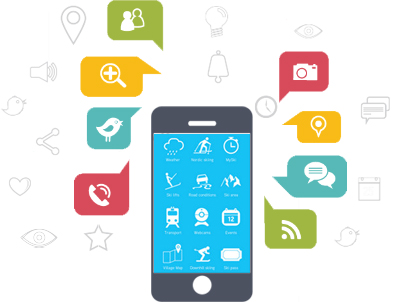
\includegraphics[width=0.4\textwidth]{images/technische_grundlagen/App-Development.jpg}
	\end{center}
	\caption{App Entwicklung}
	\label{fig:appentwicklung}
\end{wrapfigure}

Eine \gls{app} ist ein ausführbares Programm für mobile Geräte, wie Smartphones oder Tablets. Um eine \gls{app} für ein mobiles Gerät zu entwickeln, müssen wie für andere Anwendungen im Voraus Anforderungen definiert werden, die diese erfüllen soll. Je nach festgelegten Anforderungen, die an das System gestellt werden, besteht eine bestimmte Anzahl von Möglichkeiten der Entwicklung. Allgemein kennt die \gls{app} Entwicklung drei verschiedene Arten, die native, web und hybride Entwicklung, siehe \eqref{native}, \eqref{web} und \eqref{hybride}. Dabei werden verschiedene \glspl{framework} verwendet, um mit unterschiedlichsten Programmiersprachen den Aufbau der Logik zu beschreiben. Eine App besteht immer aus zwei Teile, dem \gls{ui}, das meist mit einer \gls{xml} ähnlichen Sprache beschrieben wird und dem Programmcode, der sich auf viele Klassen verteilt und die Funktionalitäten der \gls{app} beschreiben.

\subsubsection{Native \glspl{app}}\label{native}

In der Entwicklung von nativen \glspl{app} werden die direkten Ressourcen des Gerätes verwendet. Dazu gehört die Laufzeitumgebung des Betriebssystemes, Bibliotheken und Hardwareschnittstellen. Der Vorteil von einer nativen Entwicklung liegt hauptsächlich darin, dass diese für das Betriebssystem optimiert ist und die vorhandenen Schnittstellen genutzt werden können, um komplexe und rechenintensive Anwendungen zu ermöglichen.\footnote{\citep[vgl.][Unterschiede und Vergleich native Apps vs. Web Apps]{DanielWurstl.Unterschiedeund}\label{note1}}\\
Vertreter diese Entwicklung finden sich für verschiedene Betriebssysteme. Der populärste unter ihnen ist bei weitem Android mit einer nativen Java Entwicklung über Android Studio von Google. Sie besitzt aktuellen den höchsten Marktanteil und eine entsprechende Popularität unter Entwickler und Nutzer.

\subsubsection{Web \glspl{app}}\label{web}

Die Entwicklung von web \glspl{app} arbeitet mit systemübergreifenden Ressourcen und greift auf gängige Webtechnologien, wie \gls{html}, \gls{css} und \gls{javascript} zurück. Die \gls{app} wird hierbei nicht wie normale Anwendungen direkt auf dem System des Gerätes ausgeführt, sondern kommt in dessen Browser zur Ausführung. Der Vorteil hierbei ist vor allem, dass diese Art von \gls{app} auf allen Betriebssystemen lauffähig ist und direkt über das Internet veröffentlicht und aktualisiert werden kann, jedoch wird eine stabile Internetverbindung vorausgesetzt.\footref{note1}\\
Von dieser Entwicklung finden sich viele Vertreter mit der Unterstützung diverser \glspl{framework}. Das populärste unter ihnen ist aktuell AngularJS von Google, was auf \gls{javascript} basiert. In Kombination mit anderen Webtechnologien, wie \gls{html} und \gls{css} lassen sich perfomante web \glspl{app} entwickeln.

\subsubsection{Hybride \glspl{app}}\label{hybride}

Die Entwicklung von hybride \glspl{app} vereinigt die beiden Entwicklungen von native und web. Sie besteht dabei aus einem nativen Rahmen, in der eine web \gls{app} zur Ausführung kommt, diese besitzt entsprechende Zugriffsrechte auf Hardwareschnittstellen, um diese mit \glspl{api} anzusprechen.\footnote{\citep[vgl.][Native App, Web App und Hybrid App im Überblick]{PetraRiepe.NativeApp}\label{note2}}\\
Diese Entwicklung ist aktuell noch sehr jung, jedoch stechen hier bereits verschiedene Vertreter hervor. Der populärste unter ihnen ist Ionic von Drifty, welches auf Apache Cordova als Basis zurückgreift. In Kombination mit AngularJS, \gls{typescript} und anderen Webtechnologien lässt sich die web \gls{app} entwickeln und auf einem beliebigen Gerät unter einem nativen Browser ausführen. Es unterstützt dabei verschiedenste Betriebssystem, wie Android, iOS und Windows. Diese Entwicklungen können dabei meist nicht nur mobil, sondern unter anderem auf weiteren Systemen, wie stationäre bereitgestellt werden.

\subsubsection{Plattformübergreifende Entwicklung}

Um die Entwicklung von \glspl{app} einfach zu halten, verwenden immer mehr Entwickler die Form der plattformübergreifenden Entwicklung. Dadurch lässt sich die \gls{app} unabhängig des Betriebssystems entwickeln und kann somit eine größere Menge von Nutzern erreichen. Diese Entwicklung greift dabei meist auf plattformübergreifende Konzepte, wie eine native Laufzeitumgebung, oder Browser zurück, um darin die \gls{app} auszuführen. Der große Vorteil in dieser Entwicklung, liegt in der Wiederverwendbarkeit des Quellcodes und der verbesserten Wartbarkeit, da hier lediglich ein Projekt gewartet werden muss und der Quellcode für viele Betriebssysteme übernommen werden kann. Zur plattformübergreifenden Entwicklung wurden die letzten Jahre viele Ansätze mit verschiedenen \glspl{framework} entwickelt. Beispiele hierfür sind Ionic, Unity, Qt oder Xamarin.\\
\newpage

\subsubsection{Xamarin}

\begin{wrapfigure}{r}{0.3\textwidth}
	\begin{center}
		
\includegraphics[width=0.25\textwidth]{images/technische_grundlagen/xamarin.png}
	\end{center}
	\caption{Xamarin}
	\label{fig:xamarin}
\end{wrapfigure}

Xamarin ist ein \gls{framework} zur Entwicklung von nativen plattformübergreifenden Apps, welches auf Mono basiert, siehe \eqref{mono}. Um nativen Quellcode auf den verschiedenen Systemen auszuführen, setzt Xamarin auf verschiedene Softwarekomponenten, um aus einem mit .NET entwickelten Projekt nativen Quellcode zu erzeugen.\\
Für iOS Systeme verwendet Xamarin den \gls{aot} Compiler, um aus einem Xamarin.iOS Projekt \gls{arm} Maschinencode zur erzeugen, der entsprechend schnell auf dem System ausgeführt werden kann.\footnote{\citep[vgl.][Introduction to Mobile Development - Xamarin]{Xamarin.Introductionto}\label{note3}} Bei Android hingegen wird der Quellcode in \gls{il} übersetzt, welches \gls{jit} nutzt um zur Laufzeit Maschinencode für das entsprechende Gerät zu erzeugen.\footref{note3} Dazu nutzt Xamarin Softwarekomponenten, während der Laufzeit, um bestimmte Prozesse, wie Speicherverwaltung und Plattformoperationen. Zur Entwicklung bringt Xamarin eine große Bandbreite von Funktionalitäten für den Entwickler, wie Bibliotheken, eine Test Cloud, sowie Unterstützung von nativen Bibliotheken, wie für \gls{java} oder \gls{objectivc}. Xamarin bietet Unterstützung für diverse Betriebssysteme, wie zum Beispiel Android, iOS, Windows und Windows Phone. Um mit Xamarin zu entwickeln, gibt es aktuell verschiedene Möglichkeiten mit Unterstützung auf unterschiedlichen Betriebssystemen. Einerseits kann mit Xamarin Studio auf einem OSX System, oder mit Visual Studio auf Windows und Linux entwickelt werden.\\
Wie viele andere \glspl{framework}, bietet auch Xamarin verschiedene nützliche \glspl{template}, die jeweils andere Nutzen besitzen. Diese bauen dabei auf zwei Hauptkomponenten von Bibliotheken, einerseits Shared Projects und Protable Class Libraries.

\begin{wrapfigure}{r}{0.55\textwidth}
	\begin{center}
		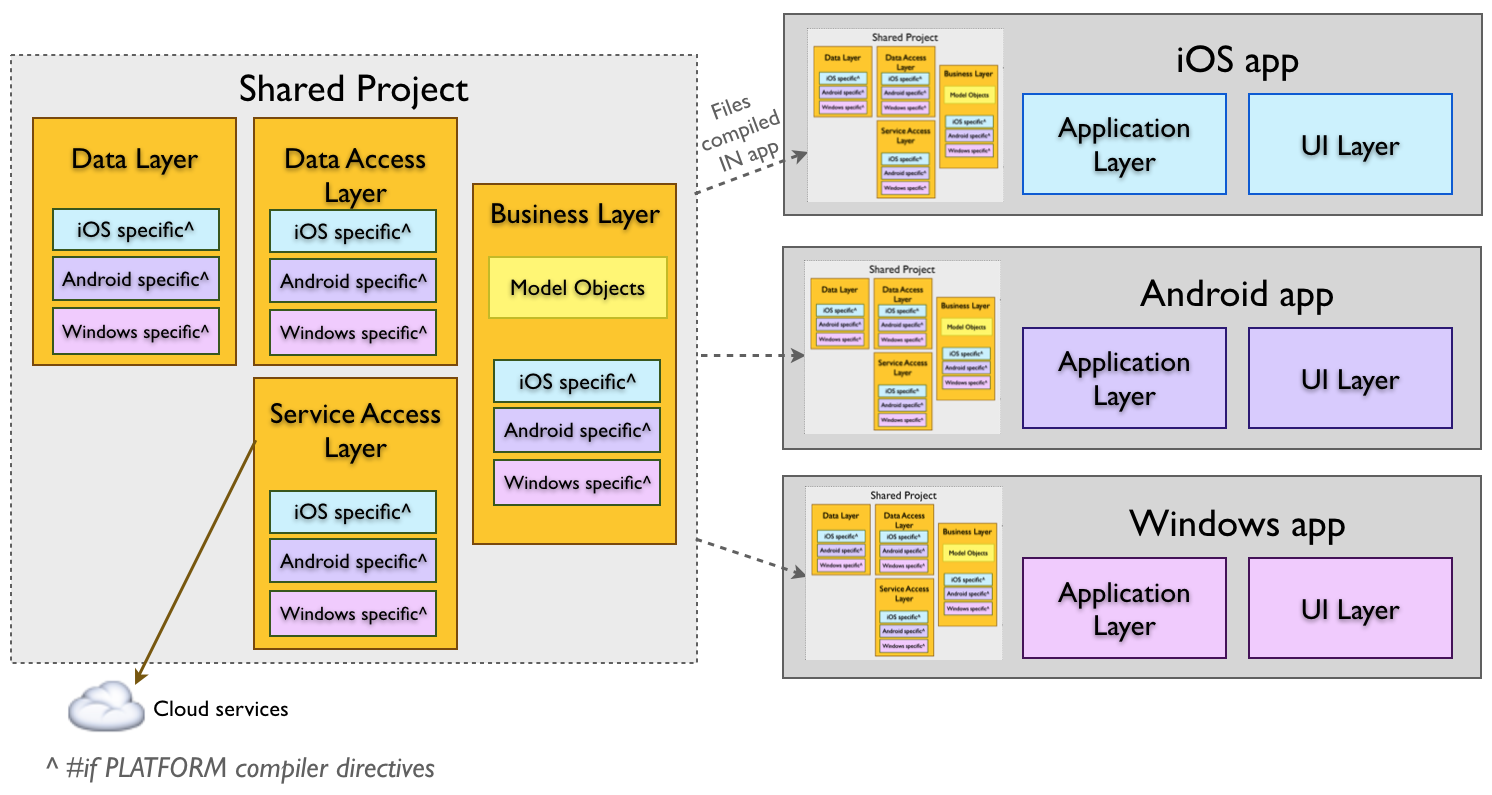
\includegraphics[width=0.5\textwidth]{images/technische_grundlagen/SharedAssetProject.png}
	\end{center}
	\caption{Shared Project}
	\label{fig:shared}
\end{wrapfigure}

\paragraph{Shared Projects}

ermöglichen dem Entwickler Quellcode für verschiedene Plattformen zu entwickeln, wobei die plattformspezifischen Projekte das entsprechende shared Project referenzieren. Somit besitzt diese Projektart keinen direkten Output, sondern kopiert den Quellcode in das zu entsprechend bauende Projekt, siehe Abbildung \eqref{fig:shared}.\footnote{\citep[vgl.][Shared Projects - Xamarin]{Xamarin.SharedProjects}\label{note4}} Der Hauptunterschied zu Standardprojekten liegt vor allem darin, dass ein shared Project keine Abhängigkeiten haben darf und daher lediglich als Referenz für andere Projekte dienen kann.

\begin{wrapfigure}{r}{0.55\textwidth}
	\begin{center}
		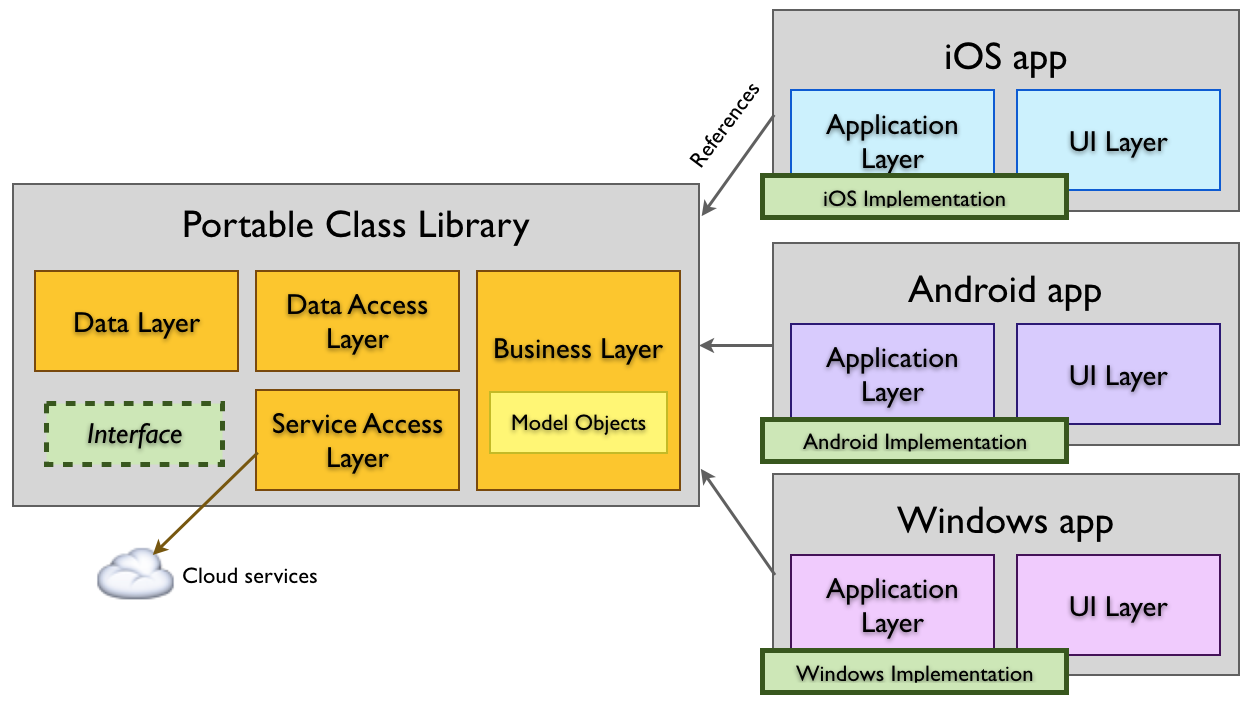
\includegraphics[width=0.5\textwidth]{images/technische_grundlagen/PortableClassLibrary.png}
	\end{center}
	\caption{Portable Class Library}
	\label{fig:portable}
\end{wrapfigure}

\paragraph{Protable Class Libraries}

ermöglichen dem Entwickler die Implementierung von plattformübergreifende Bibliotheken, aus denen \glspl{dll} erzeugt werden können. Das Besondere an Portable Class Libraries ist dabei, dass die Plattformen spezifisch ausgewählt werden können, wobei auf die Unterstützung verschiedener Betriebssysteme zu achten ist, siehe Abbildung \eqref{fig:pcl_support}.\footnote{\citep[vgl.][Introduction to Portable Class Libraries - Xamarin]{Xamarin.PortableClass}\label{note5}} Eine Portable Class Library besitzt darüber hinaus verschiedene Vor- bzw. Nachteile, die für oder Gegen ihre Nutzung sprechen.\\

\begin{wrapfigure}{r}{0.55\textwidth}
	\begin{center}
		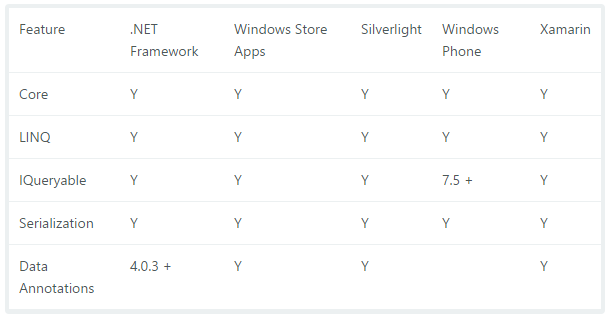
\includegraphics[width=0.5\textwidth]{images/technische_grundlagen/pclSupport.png}
	\end{center}
	\caption{Unterstützung Portable Class Library}
	\label{fig:pcl_support}
\end{wrapfigure}

\noindent
Vorteile:
\begin{itemize}
	\item Implementierung von zentralem Quellcode
	\item Einfaches Refactoring
	\item Referenzierung von Anwendungen
\end{itemize}
\noindent
Nachteile:
\begin{itemize}
	\item Keine Referenzierung von Plattform spezifischem Quellcode
	\item Keine Standardbibliotheken vorhanden
\end{itemize}

\newpage
\subsubsection{Mono}\label{mono}

\begin{wrapfigure}{r}{0.3\textwidth}
	\begin{center}
		
\includegraphics[width=0.25\textwidth]{images/technische_grundlagen/mono.png}
	\end{center}
	\caption{Mono}
	\label{fig:mono}
\end{wrapfigure}

Mono ist ein opensource Framework, das auf dem .NET Framework von Microsoft basiert. Die Implementierung von Mono greift dabei auf die Standards von .NET für die Programmiersprache \gls{csharp}, sowie die \gls{cli} zurück.\footnote{\citep[vgl.][About Mono]{MonoProject.AboutMono}\label{note6}} Dies ermöglicht Entwicklern die Erstellung von plattformübergreifenden Anwendungen, welche mittels einer zur Verfügung gestellten Laufzeitumgebung auf verschiedenen Systemen ausgeführt werden können.\\
Um Anwendungen auf verschieden Systemen auszuführen, nutzt Mono verschiedene Komponenten. Dazu gehört an vorderster Stelle ein Compiler, um den erstellten Quellcode in die jeweilige Maschinensprache zu übersetzen. Die Übersetzung findet dabei in Kooperation der Mono Runtime statt, die die entsprechende Infrastruktur zur Ausführung der Anwendung bereitstellt. Für eine effiziente Entwicklung stellt Mono zwei Bibliotheken zur Verfügung, einerseits die .NET Class Library, die die Grundelemente von .NET enthält, sowie die Mono Class Library mit zusätzlichen Funktionen für plattformübergreifende Anwendungen.\\
Für die Nutzung von Mono stehen verschiedene Vorteile im Vergleich zu anderen Framework. Der Hauptgrund für die Nutzung liegt vor allem in der Popularität von .NET, da dies auf den meisten Computern zur Verfügung steht, oder installiert werden kann. Ein großer Nutzen stellt die High-Level Programmierung dar, die eine Implementierung mit einer Laufzeitumgebung ermöglicht, die Funktionen wie Speicherverwaltung selbst organisiert. Durch Verwendung der \gls{clr} kann der Entwickler seine übliche Programmiersprache verwenden und ist unhabhängig vom bestehenden System.

\subsubsection{.NET Framework}\label{net}
%\footnote{\citep[vgl.][Overview of the .NET Framework]{Microsoft.Overviewof}\label{note7}}

Das .NET Framework dient zur Entwicklung, sowie Ausführung von Anwendungen, die mit Programmiersprachen implementiert werden, die auf den Standards von .NET basieren. Es besteht aus verschiedenen Komponenten, wobei der Kern des Frameworks in der \gls{clr} liegt. Diese ist verantwortlich für die Laufzeitumgebung und entsprechend für die Ausführung der Anwendungen, indem es die bereitgestellten Ressourcen des Systems nutzt.\\

\subsection{TCP-Kommunikation}
Das Transmission Control Protocol (TCP) ist ein Transportprotokoll und ermöglicht eine Datenaustausch zwischen kommunizierenden Anwendungsinstanzen in einer Ende-zu-Ende-Beziehung zwischen. TCP ist als Transportprotokoll auf in der 4 Schicht des OSI-Modells angesiedelt und basiert auf dem Internetprotokoll (IP) mit dem zusammen es als Nahmensgeber der TCP/IP-Protokollfamilie (Internetprotokollfamilie) dient.
TCP ist ein offenes, frei verfügbares und weit verbreitetes Protokoll. Als Mitglied der Internetprotokollfamilie ist TCP neben UDP das Transportprotokoll, auf dem die meisten Anwendungen im Internet basieren [GD189].
\subsubsection{Gundlegendes}
Als verbindungsorientiertes Protokoll sorgt TCP für die Erzeugung und Erhaltung einer gesicherten 
Ende-zu-Ende-Verbindung zwischen zwei Anwendungsprozessen. TCP arbeitet paketvermittelt d.h. überträgt Daten Paketweise und ist ein zuverlässiges Protokoll.
Durch diese Eigenschaften stellt TCP sicher dass, Daten
\begin{itemize}
	\item{nicht verloren gehen}
	\item{nicht verändert werden}
	\item{nicht dupliziert werden}
	\item{in der richtigen Reihenfolge eintreffen}
\end{itemize}
Zur Gewährleistung einer vollständingen Übertragung sowie der Integrität der gesendeten Daten nutzt TCP Prüfsummen,Bestätigungen, Zeitüberwachungs- und Nachrichtenwiederholungsmechanismen sowie Sequenznummern für die Reihenfolgeüberwachung und das Sliding Windows Prinzip zur Flusskontrolle [GD].
\newline
TCP nutzt prinzipiell folgende Protokollmechanismen:
\begin{itemize}
	\item{Drei-Wege-Handshake-Verbindungsauf- und -abbau}
	\item{Positives, kumulatives Bestätigungsverfahren mit Timerüberwachung für jede Nachricht}
	\item{Implizites negatives Bestätigungsverfahren (NAK-Mechanismus): Bei drei ankommenden Duplikat-ACK-PDUs wird beim Sender das Fehlen des folgenden Segments angenommen. Ein sog. Fast-Retransmit-Mechanismus führt zur Neuübertragung des Segments, bevor der Timer abläuft.}
	\item{Pipelining}
	\item{Go-Back-N zur Übertragungswiederholung}
	\item{Fluss- und Staukontrolle}
\end{itemize}
\subsubsection{Nagle-Algorithmus}
Nagle-Algorithmus (RFC 896 und RFC 1122) ist ein Algorithmus der der Optimierung dient und der bei allen 
TCP-Implementierungen verwendet wird. Der versuchte Nagle-Algorithmus aus Optimierungsgründen zu verhindern, dass viele kleine Nachrichten gesendet werden, da dies schlecht für die Netzauslastung ist [GD198]. \newline
Dazu werden mehrere Nachrichten zusammengefasst und gebündelt versendent, dies geschieht nach folgendem Prinzip:
\begin{itemize}
	\item{Erhält der TCP-Endpunkt Daten vom Anwendungsprozess wird zunächst nur das erste Datenpaket gesendet und die restlichen Daten werden im Sendepuffer gesammelt.}
	\item{Danach werden weiteren Daten so lange im Sendepuffer gesammelt bis alle zuvor gesendeten Datenpakete vom Empfänger bestätigt wurden oder so viele Daten im Sendepuffer liegen das die eingstellte Segmentgröße erreicht ist und ein volles Datenpaket gesendet werden kann.}
\end{itemize}
Dieses Verfahren sorgt zwar für eine gute Netzauslastung da das Verhältnis von Nutzdaten zu Overhead (TCP-Header etc.) steigt jedoch ist dies allerdings nicht nicht für alle Anwendungsszenarien optimal da es die Latenz erhöt. Insbesondere bei Anwendungen die eine ummittelbare Antwort der Gegenstelle benötigen wie SSH- oder Telnet-Anwendung sorgt dies für Verzögerungen. In diesem Fall ist es besser den Nagle-Algorithmus auszuschalten. [GD198 f.]
\subsubsection{Kommunikationsablauf}
Da es sich bei TCP um ein verbindungsorientiertes Protokoll handelt gliedert sich die Kommunikation in die drei Phasen Verbindungsaufbau, Datenaustausch und Verbindungsabbau. Bevor Daten übertragen werden können muss die Verbindung durch den Verbindungsaufbau initiert und nach Beendinung der Datenbertragung
wieder abgebaut werden. 
\paragraph{Client \& Server}
Der Verbindungsaufbau einer Kommunikation erfolgt bei TCP nach dem Client-/Server-Paradigma, d.h. einer der Teilnehmern aggiert als Server und wartet auf einen Verbindungsaufbau durch den Client welchen der andere Teilnehmern darstellt. \newline
Nach dem Verbindungsauffbau haben die beiden Rollen jedoch keine Bedeutung mehr und die beide Teilnehmern
sind sowohl bei der Datenübertragung als auch beim Verbindungsabbau gleichberechtigt.
\paragraph{Verbindungsaufbau} \code{}
\newline
\smallskip
\begin{figure}[ht]
	\centering
	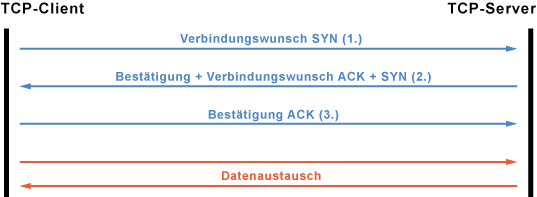
\includegraphics[width=0.8\textwidth]{images/Verbindungsaufbau.png}
	\caption[TCP Verbindungsaufbau]{TCP Verbindungsaufbau}
	\label{fig:<Sprungmakre>}
\end{figure}
Der Verbindungsaufbau bei TCP basiert auf dem Three-Way-Handshake. Dabei schickt der schickt der Client einen Verbindungswunsch (SYN) an den Server. Der Server bestätigt den Erhalt der Nachricht (ACK) und äußert seinerseits einen Verbindungswunsch (SYN) welchen der Client nach Erhalt der Nachricht bestätigt (ACK). Nach Abblauf dieses gegenseitigen Anfrage- und Bestätigugsvorgangs ist die Verbindung initiiert und der Datenaustausch zwischen den Teilnehmern kann beginnen [EK].
\paragraph{Datenaustausch}
\begin{figure}[ht]
	\centering
	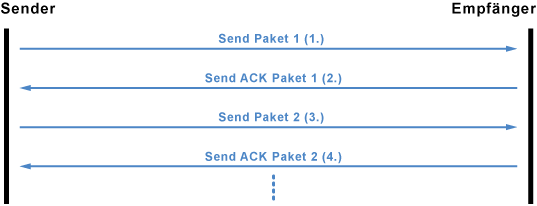
\includegraphics[width=0.8\textwidth]{images/Datenaustausch.png}
	\caption[TCP Datenaustausch]{TCP Datenaustausch}
	\label{fig:<Sprungmakre>}
\end{figure}
\paragraph{Verbindungsabbau}
\begin{figure}[ht]
	\centering
	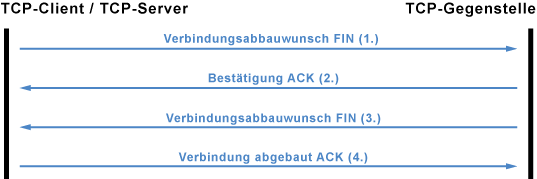
\includegraphics[width=0.8\textwidth]{images/Verbindungsabbau.png}
	\caption[TCP Verbindungsabbau]{TCP Verbindungsabbau}
	\label{fig:<Sprungmakre>}
\end{figure}
Nach Abschluss der Datenübertragung wird von einer Seite (egal von welcher) ein Verbindungsabbau initiiert. Dazu dient einen etwas modifizierten Drei-Wege-Handshake-Mechanismus. Jede der beiden Verbindungsrichtungen der Vollduplex-Verbindung wird abgebaut, d.h. beide Seiten bauen ihre „Senderichtung“ ab. Die initiierende Seite schickt zuerst einen Verbindungsabbauwunsch (FIN). Die Gegenstelle bestätigt den Erhalt der Nachricht (ACK) und schickt ebenfalls einen Verbindungsabbauwunsch (FIN) woraufhin sie von der Gegenstelle noch mitgeteilt bekommt, dass die Verbindung abgebaut ist (ACK).
\subsubsection{Socket-Programmierung}
Als Transportzugriffsschnittstelle für die TCP-basierte Kommunikation dient die Socket-Schnittstelle.
Obwohl es sich bei TCP ein paketvermitteltes Protokoll handlet der Anwendung eine Strom-orientierte Kommunikation, die Daten werden also von einem Anwendungsprozess Byte für Byte in einem Bytestrom geschrieben und TCP sorgt anschlieend um den Aufbau von Segmenten, die dann übertragen werden. Andere Transportdienste erwarten ihre Daten in festen Blöcken [GD].
\subsection{Java} %Gemeinsam ca. 2
\begin{wrapfigure}{r}{0.45\textwidth}
	\begin{center}
		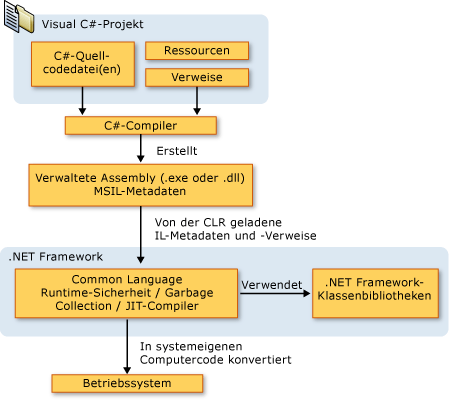
\includegraphics[width=0.4\textwidth]{images/technische_grundlagen/net_aufbau.jpeg}
	\end{center}
	\caption{.NET Framework Ausführung}
	\label{fig:net}
\end{wrapfigure}

\noindent
Die \gls{clr} führt zur Laufzeit je nach System verschiedene Aktionen aus, um die entsprechende Anwendung auszuführen. Der allgemeine Ablauf ist dabei folgender. Der Quellcode wird in die \gls{clr} geladen und nach Sicherheitsanforderungen entsprechend des Systems überprüft. Anschließend wird er durch eine \gls{jit} Kompilierung in einen \gls{il} Quellcode konvertiert, um diesen nativ auf dem System ausführen zu können. Der \gls{il} Quellcode setzt dabei auf die gesetzten Standards der \gls{cli} auf, die eine sprach- und plattformunabhängige Entwicklung von Anwendungen ermöglicht.\\
Das .NET Framework bietet zusätzlich zur unabhängigen Entwicklung verschiedene unterstützende Komponenten. Die wichtigste unter ihnen ist die .NET Class Library. Diese unterstützt den Entwickler mit einer Sammlung bereits implementierten Quellcode, wie Klassen und entsprechenden Zugang zu systemnahen Schnittstellen. Mit dem .NET Framework lässt sich eine große Bandbreite von Anwendungen entwickeln, von Konsolenanwendungen, grafischen Oberflächen, bis hin zu Webanwendungen.\\

\begin{figure}[h]
	\centering
	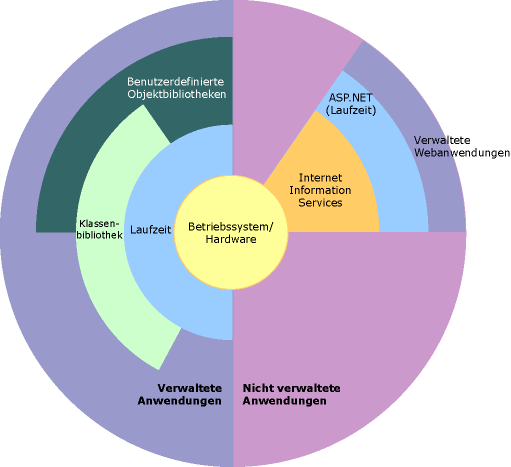
\includegraphics[width=0.65\textwidth]{images/technische_grundlagen/clr.png}
	\caption{Common Language Runtime}
	\label{fig:clr}
\end{figure}

\color{process}

\newpage
\section{Theoretische Grundlagen}

\subsection{Schwarmverhalten}
\subsubsection{Allgemein}
\subsubsection{Vorbilder aus dem Tierreich}
% Fische, Bienen, Ameisen
\subsubsection{Szenarien}
\subsubsection{Algorithmen}

%\subsection{Kommunikation} %Manuel ca. 5
%\subsubsection{Grundlagen}
%\subsubsection{TCP/IP}
%\subsubsection{Wifi}
%\subsubsection{Datenaustausch} %(JSON und Serialisierung)

	\section{Projektorganisation}
	\color{finishing}

\section{Konzeption}

In diesem Kapitel werden die Anforderungsdefinitionen des Projektes, mit Spezialisierung auf die verschiedenen Use Cases beschrieben.

\subsection{Anforderunsdefinitionen}

Ein Schwarmverhalten zur Interaktion von Kleinroboter benötigt verschiedene Anforderungen, um korrekt untereinander agieren zu können. Die Basis hierbei bildet das Kommunikationssystem zwischen den einzelnen Komponenten, um erfasste Daten zuverlässig zu synchronisieren. Um die Daten entsprechend zu interpretieren benötigt jede Komponente den jeweiligen Aufbau der Kommunikation, damit diese verwertet und Aktionen ausgeführt werden können.\\
Diese Aktionen repräsentieren den Grundbestandteil des Schwarmverhaltens und sind auf die verschiedenen Systeme verteilt. Die Roboter benötigen hierbei implementierte Funktionen, wie das Ansteuern von Motoren, Sensorik, sowie die Aktualisierung, um erfasste Daten an Nutzer weiterzuleiten. Zur Steuerung dient eine App für mobile Smartphones mit einem \gls{ui} um verschiedene Szenarien zu starten, sowie die Roboter kontrollieren zu können. Die Kontrollschnittstelle stellt dabei eine Desktopanwendung dar, über die der Nutzer mit den Robotern kommuniziert und Daten zur Steuerung abgreifen kann, wobei mehrere Nutzer zur selben Zeit mit verschiedenen Szenarien unterstützt werden sollen.\\

\noindent
Damit bestehen folgende Anforderungsdefinitionen an die zu erstellenden Softwarekomponenten:
\begin{itemize}
	\item Kommunikationssystem
	\item Interpretation
	\item \gls{ui}
	\item Steuerungsfunktionen
\end{itemize}

\newpage
\subsection{Softwarearchitektur}

Die Architektur des Schwarmverhaltens besteht aus drei Hauptkomponente, den Robotern, einer Desktopanwendung, sowie einer mobilen App, siehe Abbildung \ref{fig:softwarearchitecture}.\\
Diese Komponenten kommunizieren über ein drahtloses Netzwerk mittels \gls{tcp} untereinander, indem diese Zeichenketten als \gls{json} versenden. Dadurch lassen sich gesammelte Daten als Objekte kapseln und auf den verschiedenen Systemen entsprechend synchronisieren. Dies geschieht über eine Klassenstruktur, die Kommandos abbildet, durch die die kommunizierten Daten serialisiert und als Objekte dargestellt werden können.\\
Die Roboter basieren auf dem Java System \gls{lejos}, da durch die bereitgestellten Bibliotheken für \gls{ev3} Systeme eine unkomplizierte Implementierung von Logik möglich ist, sowie eine direkte Unterstützung von \gls{eclipse} gegeben ist, um erstellte Software zu debuggen. Die Roboter unterstützen für ein Schwarmverhalten klassische Funktionen, um die Daten der vorhandenen Sensorik auszulesen, sowie Motoren anzusteuern. Diese Funktionen werden einerseits durch Kommandos ausgeführt um den entsprechenden Roboter zu steuern. Anderseits werden regelmäßig Daten durch einen Prozess erfasst, um diese auf dem Backend zu aktualisieren.\\
Die App beruht auf der plattformübergreifenden Implementierung mittels des Frameworks Xamarin um möglichst viele Systeme zu erreichen. Sie baut dabei auf ein einfaches \gls{ui} mit dem Design Pattern \gls{mvvm} auf, um diese von der eigentlichen Logik zu trennen und einen qualitativ hochwertigen Quellcode zu schaffen, der einfach gewartet werden kann. Die App besitzt Basisfunktionen zur Erstellung von Kommandos, die die Verwaltung von Szenarien veranlassen und steuert somit den Schwarm.\\
Das Backend dient als Kommunikationsschnittstelle des gesamten Systems und steuert die Kommandos für den Ablauf der Szenarien. Es besitzt ein \gls{ui} mit \gls{javafx} Realisierung zur Anzeige von erfassten Daten der einzelnen Komponenten und stellt diese anhand einer auswählbaren Hierarchie dar.

\newpage
\begin{verbatim}
\end{verbatim}
\begin{figure}[h]
	\centering
	\includegraphics[width=0.65\textwidth]{images/konzeption/Softwarearchitecture.png}
	\caption{Softwarearchitektur}
	\label{fig:softwarearchitecture}
\end{figure}

\newpage
\subsection{Steuerung}

Die Steuerung des Roboterschwarms greift in sämtlich implementierten Szenarien auf die Sensorik des Smartphones als Basis zurück. Verwendet werden hierbei die Bewegungssensoren um eine Steuerung durch das Hin- und Herschwenken des Smartphones zu ermöglichen. Dies stellt eine intuitive Steuerung dar und ist für jeden neuen Nutzer schnell begreiflich. In Abbildung \ref{fig:steuerung} ist die entsprechende Steuerung zur Bewegung des Roboters dargestellt. Um die Roboter möglichst genau zu steuern, erfasst die Sensorik laufend Daten, welche im \gls{ui} angezeigt werden. Dadurch lässt sich eine Veränderung der Daten darstellen, die zu einer signifikant verbesserten Steuerung führen.\\

\begin{figure}[h]
	\centering
	\includegraphics[width=0.7\textwidth]{images/Controling.png}
	\caption{Steuerung}
	\label{fig:steuerung}
\end{figure}

\subsection{Szenarien}

Zum Ablauf der Software greift der Roboterschwarm auf verschieden definierte Szenarien als Kontext zurück. Diese sind in Control, Synchron, Follow, Flee und Catch untergliedert, wobei ein Single mit einem Nutzer oder einem Mehrnutzersystem als Multi unterschieden wird. Der Multi Mode dient hierbei als Erweiterung zur Software und ist im vorliegenden System nicht implementiert und kann daher nicht genutzt werden. Folgend werden die einzelnen Szenarien beschrieben, die als Kontext für ein Schwarmverhalten genutzt werden können.

\paragraph{Control}

stellt eine direkte Steuerung eines einzelnen Roboters und fällt somit nicht unter die Kategorie Schwarmverherhalten. Dieses Szenario dient zur Entwicklung der grundlegenden Funktionen, auf denen das Schwarmverhalten und damit weitere Szenarien aufbauen.

\paragraph{Synchron}

stellt eine synchrone Steuerung von mehreren Robotern dar, in dessen Kontext jeder beteiligte Roboter identische Kommandos erhält. Durch eine entsprechende Aufstellung der Roboter lassen sich Schwärme aus dem Tierreich, wie Fische oder Vögel nachahmen.

\paragraph{Follow}

stellt eine Reihe von Robotern dar, indem der vorderste vom Nutzer gesteuert werden kann. Die restlichen Roboter erhalten ihrer Position in der Schlange entsprechend der Position ihres Vordermannes, zu dem diese vollkommen autonom fahren. Da diese Ablauf laufend wiederholt wird, stellen alle Roboter gesamt eine Schlange dar, wobei die einzelnen die Muskeln und der vorderste Roboter den Kopf repräsentiert.

\paragraph{Flee}

stellt ein Verfolgungsszenario dar, indem der Nutzer mit seinem Roboter vor anderen flieht. Dabei erhalten die restlichen Roboter laufend eine Position um immer näher an diesen heranzufahren. Sollte der Nutzer durch einen Roboter erwischt werden, ertönt ein Endsignal , wobei anschließend das Szenario beendet wird.

\paragraph{Catch}

stellt ein Verfolgungsszenario dar, indem der Nutzer die restlichen Roboter fängt. Diese fahren zufällig in verschiedene Richtungen davon. Sollte der Nutzer alle gefangen haben, ertönt ein Signal und beendet damit das Szenario.

\begin{figure}[h]
	\begin{center}
		
\includegraphics[width=0.4\textwidth]{images/logos/UWP/FleeAndCatch_Logo.png}
	\end{center}
	\caption{Logo}
	\label{fig:Logo}
\end{figure}

\newpage
\subsection{Use Cases}

In diesem Abschnitt werden die Use Cases des Schwarmverhaltens beschrieben. Dabei wird insbesondere auf den Ablauf in Form von \gls{uml} Diagrammen eingegangen.

\subsubsection{Connection}

Der Use Case Connection stellt den Ablauf eines Verbindungsaufbaus zwischen den Komponenten und der Desktopanwendung dar. Dies soll über die Nutzung eines drahtlosen Netzwerks mittels \gls{tcp} Schnittstelle des Smartphones realisiert werden. Die IP-Adresse kann dabei durch die Verwendung einer \gls{sqlite} Datenbank lokal gespeichert werden, um diese später bei einem erneuten Aufruf automatisch eintragen zu lassen. Zur Unterscheidung der verschiedenen Komponenten soll eine individuelle Identifikation erstellt werden, wobei der Typ der Komponente, sowie weitere Merkmale ersichtlich werden sollen.\\
Der Use Case soll dabei in zwei unterschiedliche Typen untergliedert werden, womit ein Verbindungsaufbau von einem Verbindungsabbau unterschieden werden kann. Der Ablauf eines Verbindungsaufbaus soll dabei für jede Komponente identisch 
abgewickelt werden, siehe Abbildung \ref{fig:UC_Connect}. Um eine entsprechend stabile Reaktionszeit der teilnehmenden Roboter zu garantieren, sollen zum Start des Verbindungsaufbaus wiederholt Kommandos versendet werden. Dies soll eine erhöhte \gls{cpu} Laufzeit erreichen, um eine Zeitverzögerung zur Laufzeit der Szenarios zu verhindern.\\

\begin{figure}[h]
	\centering
	\subfloat[Log in]{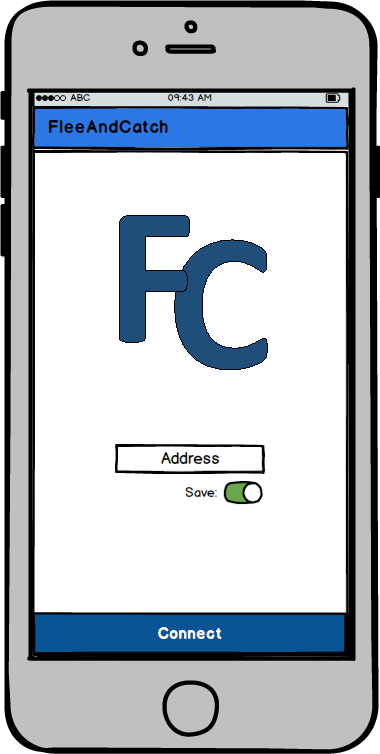
\includegraphics[width=0.25\textwidth]{images/mockups/Connection.png}\label{fig:Connect}}
	\qquad
	\subfloat[Home]{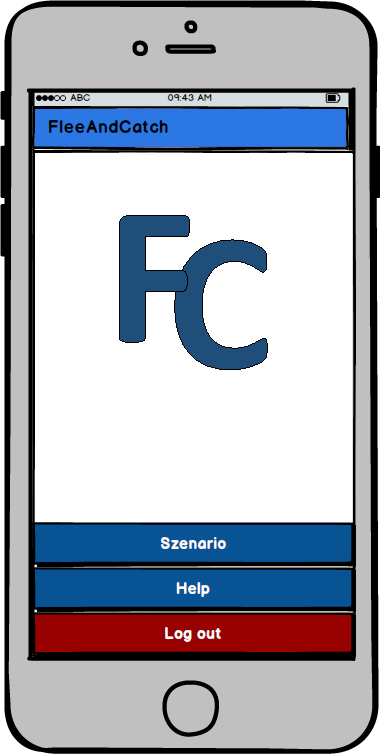
\includegraphics[width=0.25\textwidth]{images/mockups/Home.png}\label{fig:Home}}
	\caption{Mockup Connection}
\end{figure}
\newpage
\begin{verbatim}
\end{verbatim}
\begin{figure}[h]
	\begin{center}
		\includegraphics[width=1\textwidth]{images/use_cases/Connect.png}
	\end{center}
	\caption{Use Case Connection}
	\label{fig:UC_Connect}
\end{figure}

\newpage
\subsubsection{Synchronization}

Der Use Case Synchronization stellt den Datenaustausch der beteiligten Komponenten dar, siehe Abbildung \ref{fig:UC_Synchronization} und \ref{fig:UC_Update}. Hierbei sollen verschiedene Typen unterschieden werden, wobei der komplette Datensatz in Form von allen Szenarien, Robotern, oder eines einzelnen Szenarios, sowie Roboters übertragen werden soll. Dies wird einerseits der Erstellung eines Szenarios dienen, als auch dessen Beobachtung durch den Spectator Modus. Die Übertragung eines einzelnen Roboter dient der Aktualisierung der jeweiligen Daten der Desktopanwendung, sowie der App, um diese laufend aktuell zu halten. Die synchronisierten Daten sollen des Weiteren auf den Komponenten über eine \gls{ui} dargestellt werden können, um die Veränderung der aktuellen Daten zu verdeutlichen, sowie eine verbesserte Steuerung schaffen.\\

\begin{figure}[h]
	\centering
	\subfloat[Log in]{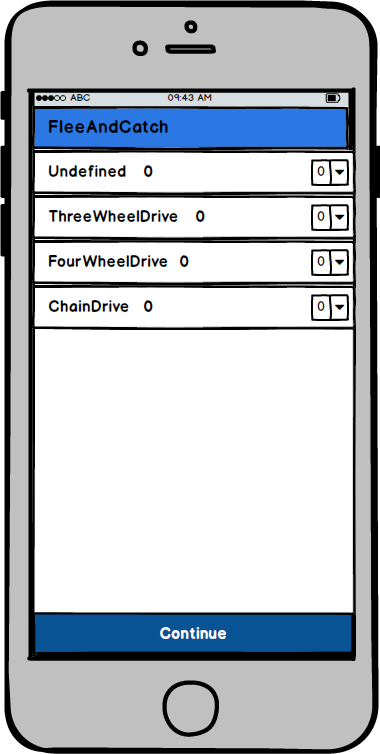
\includegraphics[width=0.25\textwidth]{images/mockups/RobotList.png}\label{fig:Synchronization_1}}
	\qquad
	\subfloat[Home]{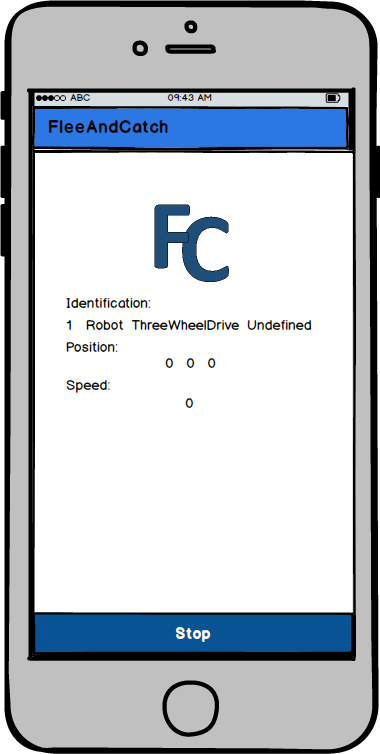
\includegraphics[width=0.25\textwidth]{images/mockups/Control.png}\label{fig:Synchronization_2}}
	\caption{Mockup Synchronization}
\end{figure}
\newpage
\begin{verbatim}
\end{verbatim}
\begin{figure}[h]
	\begin{center}
		\includegraphics[width=0.35\textwidth]{images/use_cases/Synchronization.png}
	\end{center}
	\caption{Use Case Synchronization}
	\label{fig:UC_Synchronization}
\end{figure}
\begin{figure}[h]
	\begin{center}
		\includegraphics[width=0.3\textwidth]{images/use_cases/Update.png}
	\end{center}
	\caption{Use Case Update}
	\label{fig:UC_Update}
\end{figure}

\newpage
\subsubsection{Szenario}

Der Use Case Szenario stellt den Ablauf der definierten Szenarien, zur Steuerung der Roboter dar, siehe Abbildung \ref{fig:UC_Szenario_1}. Der Nutzer soll dabei zu Beginn das gewünschte Szenario, sowie die teilnehmenden Roboter festlegen. Anschließend wird das Szenario durch das Senden eines Kommandos gestartet, welches von der Desktopanwendung initialisiert wird. Dieses Kommando soll laufend wiederholt werden, um aktuelle Daten, wie Steuerungsinformationen an die Roboter weiterzuleiten. Zur Steuerung sollen hierbei eine direkte von einer positionsorientierten unterschieden werden, wobei die Roboter je nach Kommando die direkten Steuerungsinformationen oder eine anzufahrende Position erhalten.\\
Diese Implementierung soll den Vorteil einer Auslagerung der Programmlogik schaffen, indem die Ressourcen der Roboter geschont werden und die Logik zentral in der Desktopanwendung ausgeführt werden kann.\\
 
\begin{figure}[h]
	\centering
	\subfloat[Szenario]{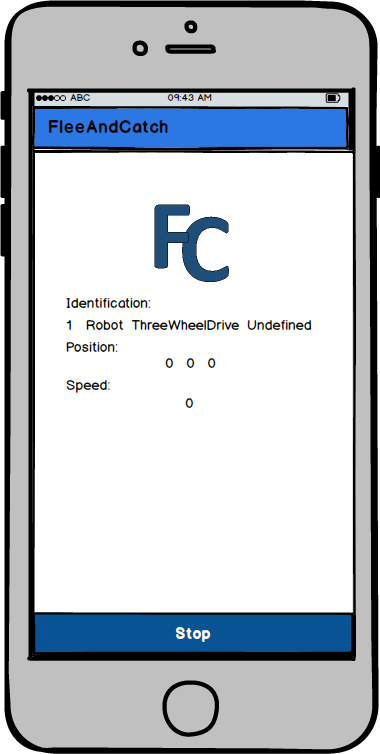
\includegraphics[width=0.25\textwidth]{images/mockups/Control.png}\label{fig:Szenario_1}}
	\qquad
	\subfloat[Spectator]{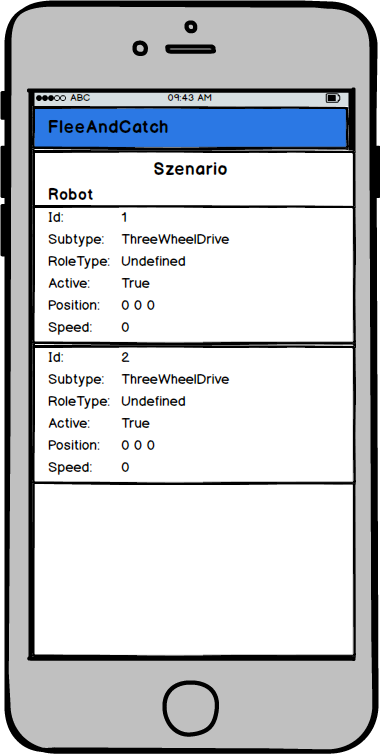
\includegraphics[width=0.25\textwidth]{images/mockups/Spectator.png}\label{fig:Szenario_2}}
	\caption{Mockup Szenario}
\end{figure}
\newpage
\begin{verbatim}
\end{verbatim}
\begin{figure}[h]
	\begin{center}
		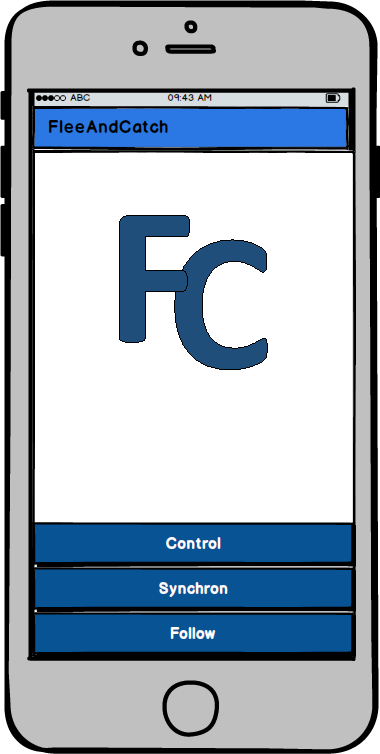
\includegraphics[width=0.425\textwidth]{images/use_cases/Szenario.png}
	\end{center}
	\caption{Use Case Szenario}
	\label{fig:UC_Szenario_1}
\end{figure}
\begin{figure}[h]
	\begin{center}
		\includegraphics[width=0.375\textwidth]{images/use_cases/Spectator.png}
	\end{center}
	\caption{Use Case Spectator}
	\label{fig:UC_Szenario_2}
\end{figure}

\newpage
\color{process}
\subsubsection{Exception}

Der Use Case Exception stellt den Ablauf einer auftretenden Exception in einem Roboter zum Kontext eines Verbindungsverlustes dar, siehe Abbildung \ref{fig:Exception}. Dabei soll die auftretenden Nachricht, sowie die beteiligte Komponente der Desktopanwendung zugesendet werden. Dies soll ein kontrolliertes Schließen eines Szenarios ermöglichen, welches von einer solchen Exception betroffen ist. Die dabei teilnehmenden Komponenten, wie Nutzer und andere Roboter sollen entsprechend zurückgesetzt werden, damit diese für ein neues Szenario zur Verfügung stehen.\\

\begin{figure}[h]
	\begin{center}
		\includegraphics[width=0.5\textwidth]{images/use_cases/Exception.png}
	\end{center}
	\caption{Use Case Exception}
	\label{fig:Exception}
\end{figure}

\newpage
\subsection{Kommunikation}
	\section{Konzeption}
	\section{Implementierung}

In diesem Kapitel wird die Implementierung des Projektes mit Fokussierung auf die einzelnen Komponenten beschrieben.

\subsection{Kommunikation}

Die Kommunikation der einzelnen Komponenten des Schwarmverhaltens baut auf einer klar definierten Struktur, um ein verteiltes System zu ermöglichen, siehe Abbildung \ref{fig:full_classdiagram}. Die Daten werden dabei als \gls{json} Objekte zur optimalen plattformübergreifenden Interpretation versendet, wobei jeweils die entsprechende Bibliothek zur Serialisierung verwendet wird.
\begin{verbatim}
\end{verbatim}
\begin{figure}[h]
	\begin{center}
		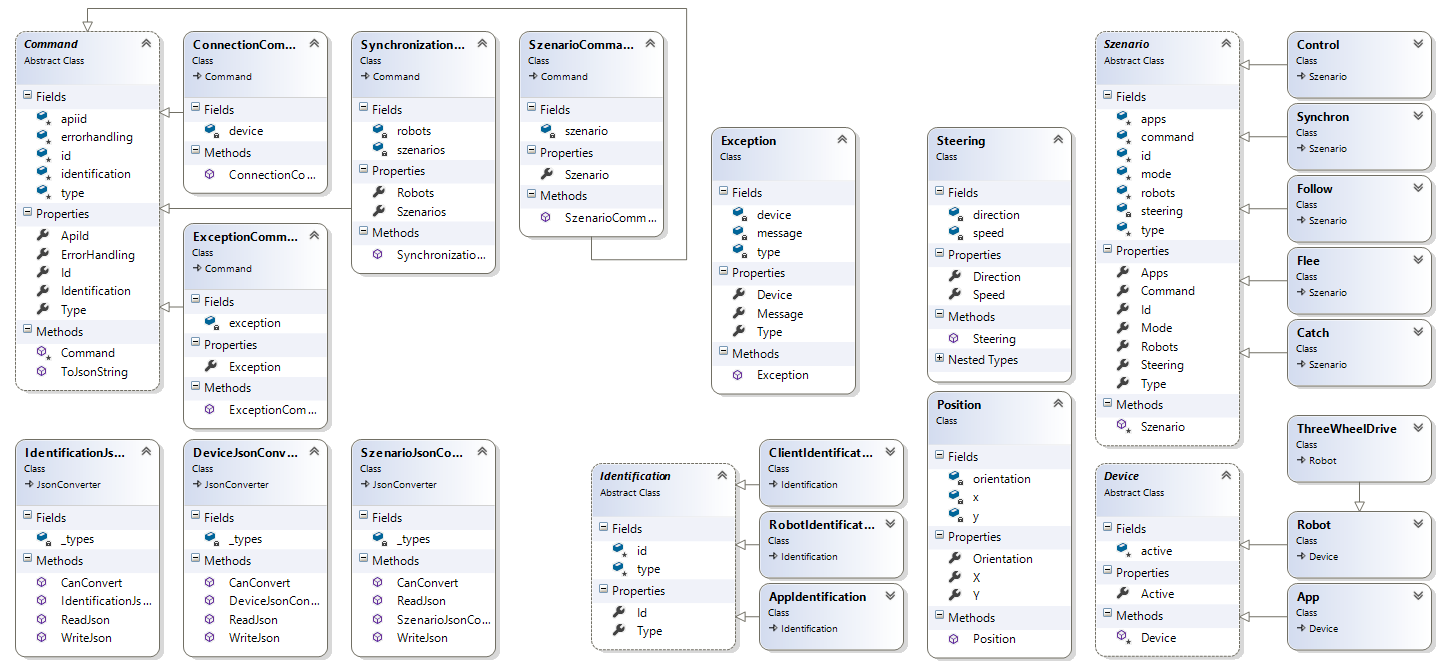
\includegraphics[width=0.95\textwidth]{images/uml/full_class_diagram.png}
	\end{center}
	\caption{Aufbau Commands}
	\label{fig:full_classdiagram}
\end{figure}

\newpage
\noindent
Der Kern zur Implementierung der Kommunikation erfolgt in zwei Methoden, die auf jeder Komponente zur Verfügung stehen. Diese dienen zum Versenden, sowie Empfangen von Daten, wobei diese als Zeichenkette serialisiert und in Bytes aufgeteilt werden, siehe Abbildung \ref{fig:SendCommand}. Um den vollständigen Umfang der Daten zu erfassen, wird die Größe ermittelt und standardmäßig mittels vier Bytes übertragen. Dadurch ist eine maximale Paketgröße von 32 Byte möglich, was einer Länge von etwa 4 Milliarden Zeichen entspricht. Die Interpretation zum Empfangen erfolgt mit ähnlichem Muster, indem zunächst die Größe der Daten festgestellt wird und die Daten deserialiert werden, siehe Abbildung \ref{fig:ReceiveCommand}.

\begin{figure}[h]
	\centering
	\subfloat[Versende Kommando]{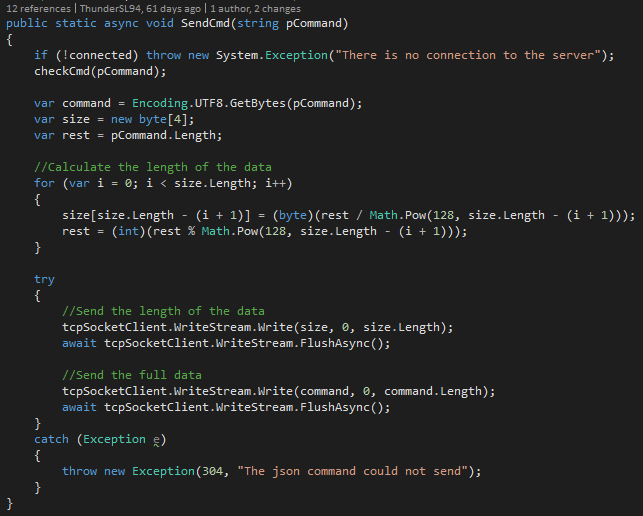
\includegraphics[width=0.6\textwidth]{images/code/SendCommand.png}\label{fig:SendCommand}}
	\qquad
	\subfloat[Empfange Kommando]{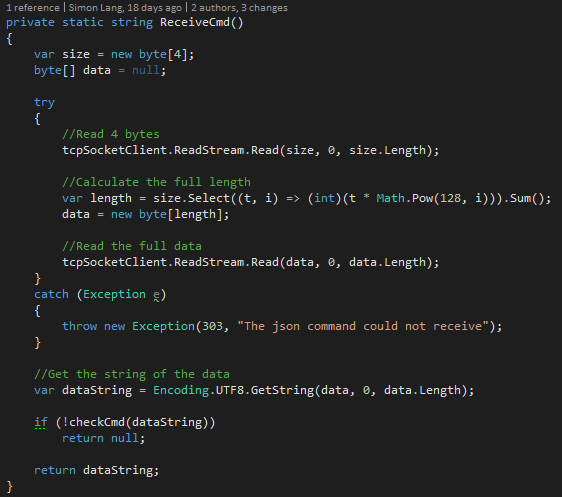
\includegraphics[width=0.6\textwidth]{images/code/ReceiveCommand.png}\label{fig:ReceiveCommand}}
	\caption{Kommunikation}
\end{figure}

\newpage
\paragraph{Kommandos}

\begin{wrapfigure}{r}{0.55\textwidth}
	\begin{center}
		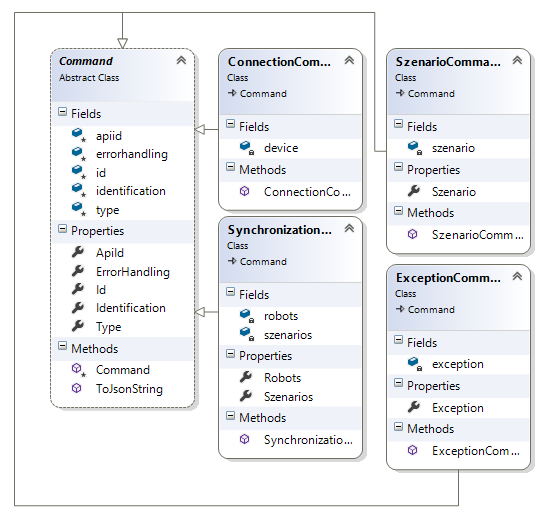
\includegraphics[width=0.5\textwidth]{images/uml/commands.png}
	\end{center}
	\caption{Kommandos}
	\label{fig:commands_classdiagram}
	\begin{center}
		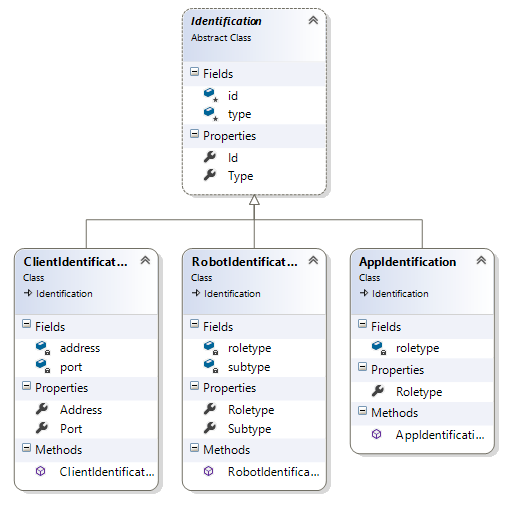
\includegraphics[width=0.5\textwidth]{images/uml/identification.png}
	\end{center}
	\caption{Identifikation}
	\label{fig:identification_classdiagram}
\end{wrapfigure}

stellen die Basis der Kommunikationsstruktur sowie den aktuellen Kontext dar, indem sich die Software befindet, siehe Abbildung \ref{fig:commands_classdiagram}. Sie enthalten grundlegende Attribute zur allgemeinen Identifikation des Kommandos, die zur Interpretation verwendet, welche über definierte Enums ausgewählt werden. Je nach Kommando sind zusätzliche Objekte enthalten, die durch die jeweilige Id vordefiniert sind.\\

\paragraph{Identifikationen}

stellt die individuelle Identität der einzelnen Komponente dar, siehe Abbildung \ref{fig:identification_classdiagram}. Diese wird durch eine fortlaufende Identifikationsnummer, Typen und je nach Ableitung weiteren Attributen erreicht. Um die jeweiligen Kommandos entsprechend zuzuordnen, sind diese in jedem Kommando vorhanden und bilden die Basisobjekte. Die unterschiedlichen Typen sind dabei für verschiedene Kontexte der Software zuständig. Die ClientIdentification stellt einerseits die Verbindung einer allgemeinen Komponente zur Desktopanwendung dar, wogegen die Robot- bzw. AppIdentification die spezifische Identifikation der Komponente darstellt. Die Erstellung der Identifikation erfolgt wiederholt zur Anmeldung der Komponente am System. Zunächst wird ein leeres Objekt erzeugt, dass anschließend durch abfragende Kommandos an die entsprechende Komponente befüllt wird, welche hinterher eine berechnete Identifikationsnummer erhält.

\newpage
\paragraph{Geräte}

\begin{wrapfigure}{r}{0.55\textwidth}
	\begin{center}
		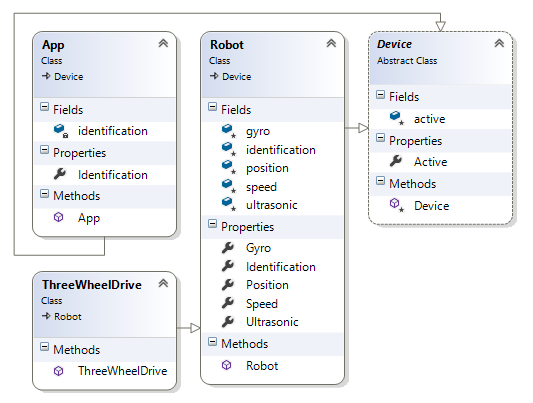
\includegraphics[width=0.5\textwidth]{images/uml/devices.png}
	\end{center}
	\caption{Devices}
	\label{fig:devices_classdiagram}
	\begin{center}
		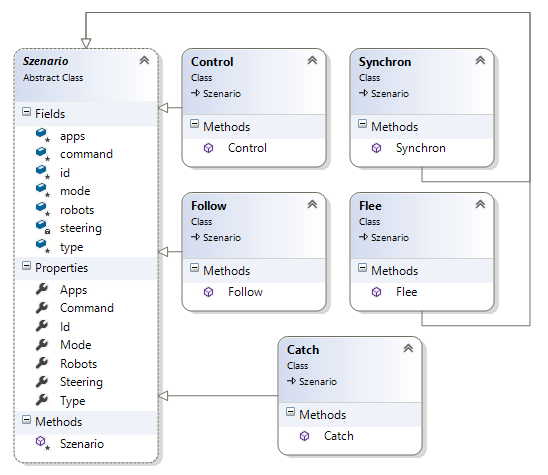
\includegraphics[width=0.5\textwidth]{images/uml/szenarios.png}
	\end{center}
	\caption{Scenarios}
	\label{fig:szenarios_classdiagram}
\end{wrapfigure}

stellen die Komponenten dar, die an einem Szenario eines Schwarmverhaltens teilnehmen, siehe Abbildung \ref{fig:devices_classdiagram}. Sie enthalten jeweils spezifische Identifikations Objekte, zur gegenseitigen Zuordnung, sowie die erfassten Daten der entsprechenden Systeme. Die Unterscheidung erfolgt in zwei Komponenten, dem Robot und der App, wobei der Roboter in die jeweiligen Untertypen gegliedert werden kann. 

\paragraph{Szenarios}

stellen den Ablauf des Schwarmverhaltens dar, in dem sich der Nutzer befindet, siehe Abbildung \ref{fig:szenarios_classdiagram}. Sie enthalten die jeweiligen Teilnehmer des Szenarios, sowie die Steuerungsinformationen und damit die gesamten Daten des aktuellen Kontextes. Diese Objekte werden laufend aktualisiert und besitzen lediglich zur Laufzeit des Szenarios ihre Gültigkeit. Dabei existieren verschiedene Kategorien von Szenarien, siehe Abschnitt \ref{szenarien}. Diese definieren jeweils einen unterschiedlichen Kontext und besitzen daher je nach Szenario zusätzliche Attribute.

\newpage
\paragraph{Konverter}

\begin{wrapfigure}{r}{0.55\textwidth}
	\begin{center}
		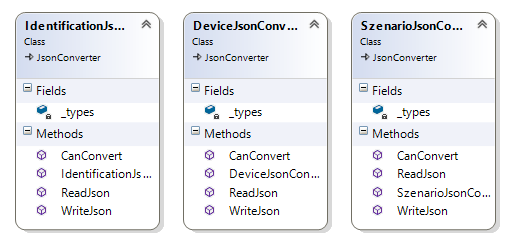
\includegraphics[width=0.5\textwidth]{images/uml/json_converter.png}
	\end{center}
	\caption{JsonConverter}
	\label{fig:converter_classdiagram}
\end{wrapfigure}

dienen der Deserialisierung von abstrakten \gls{json} Objekten, welche nicht direkt identifiziert werden können, siehe Abbildung \ref{fig:converter_classdiagram}. Dazu gehören abstrakte Klassen, sowie Schnittstellen, welche keinem spezifischen Objekt zugeordnet werden kann. Die Implementierung erfolgt durch die Überschreibung der entsprechenden Methoden zur Deserialisierung und Serialisierung, siehe Abbildung \ref{fig:ConverterRead} und \ref{fig:ConverterWrite}. Je nach Anwendung, wird ein Parameter übergeben, der das Objekt als Zeichenkette beinhaltet. Dieses wird durch eine Abfolge von Bedingungen auf den Typen geprüft wird, um das Objekt zu erstellen.\\

\begin{figure}[h]
	\centering
	\subfloat[ReadJson]{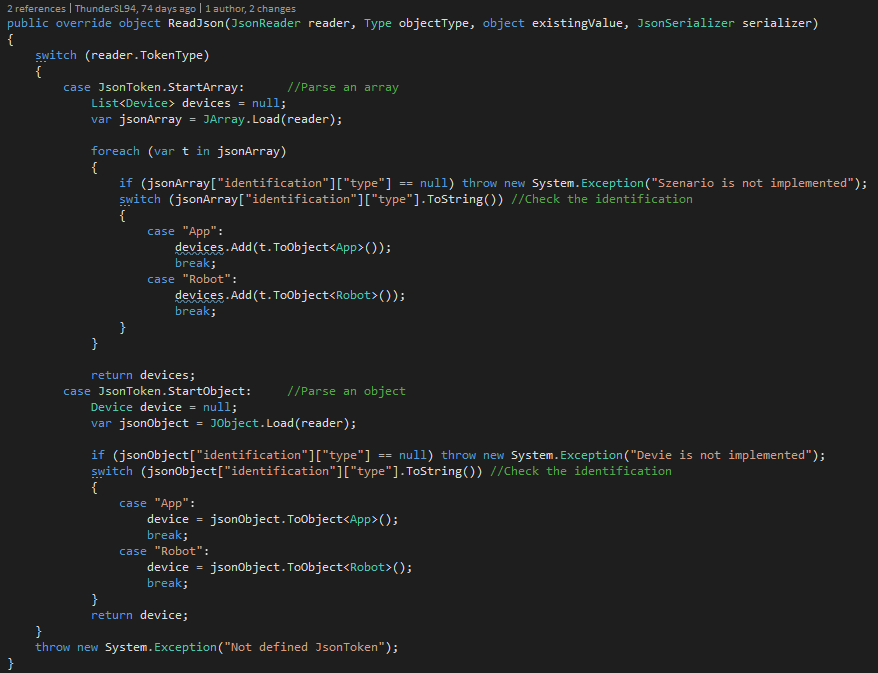
\includegraphics[width=0.6\textwidth]{images/code/DeviceConverterRead.png}\label{fig:ConverterRead}}
	\qquad
	\subfloat[WriteJson]{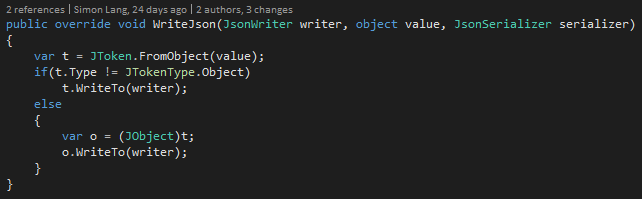
\includegraphics[width=0.6\textwidth]{images/code/DeviceConverterWrite.png}\label{fig:ConverterWrite}}
	\caption{Device JsonConverter}
\end{figure}

\newpage
\subsection{\gls{app}}

Die Erstellung der App erfolgt in einer plattformübergreifenden Implementierung durch Xamarin in C\#. Kernelemente stellen hierbei die Struktur, Oberfläche, Businesslogik sowie das Kommunikationssystem dar. Durch die zentrale Verwendung des Kommunikationssystems wird dieses in ein separates Projekt untergliedert, siehe Abbildung \ref{fig:solution} und wird als solches von der \gls{app} als Bibliothek eingebunden. Somit lässt sich die Logik einmalig implementieren und kann auf andere Systemen entsprechend übertragen werden.\\
Die \gls{app} setzt sich aus vier verschiedenen Projekten zusammen, einer \acrshort{pcl} als Projekt zur plattformübergreifenden Entwicklung und den plattformspezifischen Projekten. Diese werden dem Zielsystem entsprechend ausgewählt und erzeugen durch ihre bestehende Referenz auf die \acrshort{pcl} einen plattformspezifischen Quellcode als \gls{il}, der anschließend ausgeführt werden kann.\\

\begin{figure}[h]
	\begin{center}
		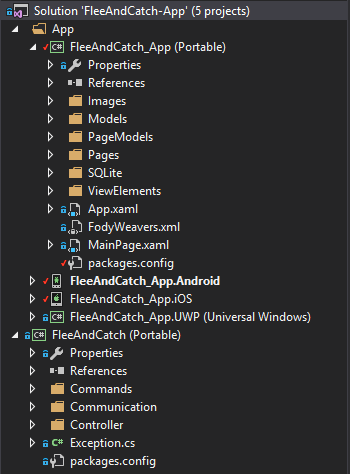
\includegraphics[width=0.5\textwidth]{images/implementation/solution.png}
	\end{center}
	\caption{Projektstruktur}
	\label{fig:solution}
\end{figure}

\newpage
\subsubsection{Workflow} %Struktur

Die Struktur der \gls{app} basiert auf dem in Xamarin verbreiteten Design Pattern \acrlong{mvvm}, welches durch ein Benachrichtigungssystem zwischen den verschiedenen Strukturen der \gls{app} eine Abspaltung der Daten, \gls{gui} und dem Businesscode erlaubt. Zusätzlich wird die standardmäßig vorhandene CodeBehind Struktur der einzelnen Seiten verwendet, wobei der Businesscode an das Layout der Seite gebunden ist, um diese miteinander zu verbinden. Zur lokalen Speicherung der Daten wird SQLite durch eine implementierte Schnittstelle verwendet, welche plattformübergreifend ansprechbar ist.

\paragraph{\acrfull{mvvm}}

stellt ein Design Pattern dar, welches eine grundlegende Struktur im Quellcode ermöglicht, siehe Abbildung \ref{fig:mvvm}. Dabei wird die erstellte Benutzeroberfläche von der Logik, sowie den Daten getrennt, um Änderungen unabhängig voneinander durchführen zu können. Die einzelnen Objekte werden dabei durch Referenzen verbunden um diese durch Events entsprechend zu aktualisieren.\\

\begin{tabular}{p{2.5cm} p{12.25cm}}
	\textbf{Model:} & Datenschicht, welche durch den Benutzer über die \gls{gui} verändert werden kann und über Datenänderungen die entsprechenden Elemente benachrichtigt \\
	\textbf{View:} & \gls{gui} mit den anzuzeigenden Elementen, welche an das ViewModel gebunden sind und der Benutzerinteraktion dienen. \\
	\textbf{ViewModel:} & Logik des \gls{ui} als zentrale Schnittstelle zwischen dem Model und der View zum Austausch von Informationen, indem entsprechende Methoden und Dienste ausgeführt werden. \\
\end{tabular}

\bigskip

\begin{figure}[h]
	\begin{center}
		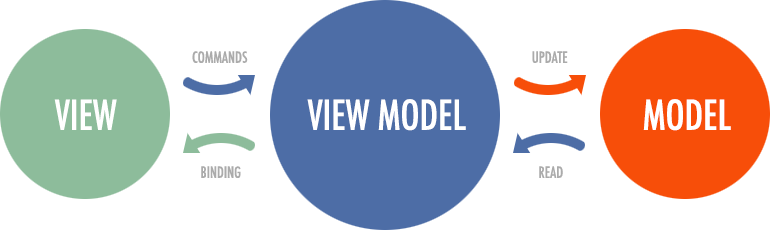
\includegraphics[width=0.95\textwidth]{images/implementation/mvvm.png}
	\end{center}	
	\caption{\acrlong{mvvm} \cite{Brecht.MVVMEntity}}
	\label{fig:mvvm}
\end{figure}

\newpage
\subsubsection{\acrfull{gui}} %Oberfläche

Die Oberfläche der \gls{app} wird mittels \gls{xaml} durch verschiedene von Xamarin zur Verfügung gestellten Elementen realisiert. Da eine \gls{app} ein einfaches Bedienkonzept voraussetzt, damit es von jedem beliebigen Benutzer verwendet werden kann,


Dabei wird für das Layout der einzelnen Seiten vor allem auf ein StackLayout gesetzt. Dieses ist sehr einfach umzusetzen, indem eine Orientierung zur Anordnung der verschiedenen Elemente festgelegt wird, welche anschließend nacheinander eingefügt werden. 




 Dabei wird für die Navigation der einzelnen Seiten vor allem auf die Verwendung der NavigationPage sowie zur Auswahl des Szenarios auf ein Carousel gesetzt. 




 mit den Aufbau eines STacks durch pushund pop aufrufe die entsprechenden Seiten gewechselt werden, siehe Abbildung xx. 

\begin{comment}
	Die Oberfläche der \gls{app} wird mittels \gls{xaml} realisiert. Dabei werden die einzelnen Elemente untereinander in der typischen \gls{xml} Struktur angeordnet und stellen damit die \gls{gui} dar, welche die einzelnen Elemente zur Benutzerinteraktion beinhaltet. Zur Strukturierung des Design bietet Xamarin verschiedene Arten von Layouts, wobei diese \gls{app} auf die Stacklayout zur Struktureirung und einer NavigationPage zur Naviagtion, sowie einem Carousel der Szenario auswahl setzt.
\end{comment}

\begin{comment}
	Die Oberfläche der \gls{app} wird mittels XAML erstellt, welche auf der Basis von XML ist. Dabei werden die einzelnen ELemente untereinnander Strukturuert, wobei der ENtwickler in Xamarin verschiedene Möglichkeiten des Designs besitzt. Grundlegend ist die entscheidung, ob eine plattformspezifisches Design sinnn macht, oder aber ein plattformübergreifendes, wobei dieses weniger Freiheiten bietet. Die plattformübergreifendes Design besitzt eine Reihe von grundlegeneden Layouts, die für Xamamrin eingesetzt werden können, sowie unterschiedliche Seitenarten. Views
	Seiten (ContentPage, MasterDetailPage, NavigationPage, TabbedPage, TemplatedPage, CaruselPage)
	View (ContentPresenter, ContentVIew, ScrollVIew, Frame, TemplatedVIew)
	Layout (Stacklayout, absolutLayout, RelativeLayout, GridLayout)
	
	Weitere standardelemente
	
	Durch verschiednene Packages könenn dabei viele Zusätzliche DInge erstellt werden
\end{comment}


%General, XAML stuff

\begin{figure}[h]
	\begin{center}
		
\includegraphics[width=0.75\textwidth]{images/implementation/push.png}
	\end{center}	
	\caption{Wechsel auf neue Seite}
	\label{fig:push}
	\begin{center}
		
\includegraphics[width=0.75\textwidth]{images/implementation/pop.png}
	\end{center}	
	\caption{Wechsel auf alte Seite}
	\label{fig:pop}
\end{figure}

\paragraph{SignIn Page} stellt die Benutzerschnittstelle zur Anmeldung des Nutzers am System dar, siehe Abbildung \ref{fig:signin}. Dabei gibt dieser die entsprechende IP-Adresse der laufenden Desktopanwendung zur Verbindung an. Durch eine implementierte Logik wird diese IP-Adresse auf ihre Richtigkeit geprüft und die Verbindung gestartet. Bei einer erfolgreichen Verbindung wird der Benutzer zur \gls{app} weitergeleitet, wodurch ihm die entsprechenden Funktionalitäten zur Verfügung stehen. Andernfalls erscheint nach einem definierten Timeout eine Fehlermeldung, welche dem User Informationen vorlegt. Zur Speicherung der IP-Adresse ist zusätzlich die Möglichkeit durch ein Switch Element gegeben, wobei diese bei Start der \gls{app} automatisch eingefügt wird.

\begin{figure}[h]
	\begin{center}
		
\includegraphics[width=0.4\textwidth]{images/implementation/signin.png}
	\end{center}	
	\caption{SignIn Page}
	\label{fig:signin}
\end{figure}

\paragraph{Home Page} stellt die Hauptseite mit der grundlegenden Navigation der \gls{app} dar, indem der Benutzer die Möglichkeit besitzt ein neues Szenario eines Schwarmverhaltens zu starten, Informationen über die \gls{app} abzurufen, oder sich vom aktuelles System abzumelden.

\begin{figure}[h]
	\begin{center}
		
\includegraphics[width=0.4\textwidth]{images/implementation/home.png}
	\end{center}	
	\caption{Home Page}
	\label{fig:home}
\end{figure}

\newpage
\paragraph{Option Page} stellt die Benutzerschnittstelle dar, welche diesen durch die vorhandenen Szenarien anhand eines Carousels leitet und ein entsprechends auswählt.

\begin{figure}[h]
	\begin{center}
		
\includegraphics[width=0.4\textwidth]{images/implementation/option.png}
	\end{center}	
	\caption{Option Page}
	\label{fig:option}
\end{figure}

\newpage
\paragraph{List Page} stellt die Benutzerschnittstelle zur Auswahl der Robotern, welche im Szenario involviert werden sollen. Dabei kann der Benutzer unter den verschiedenen Typen wählen, welche vorhanden sind, wobei die Anzahl der Roboter vom gewählten Szenario abhängt.

\begin{figure}[h]
	\begin{center}
		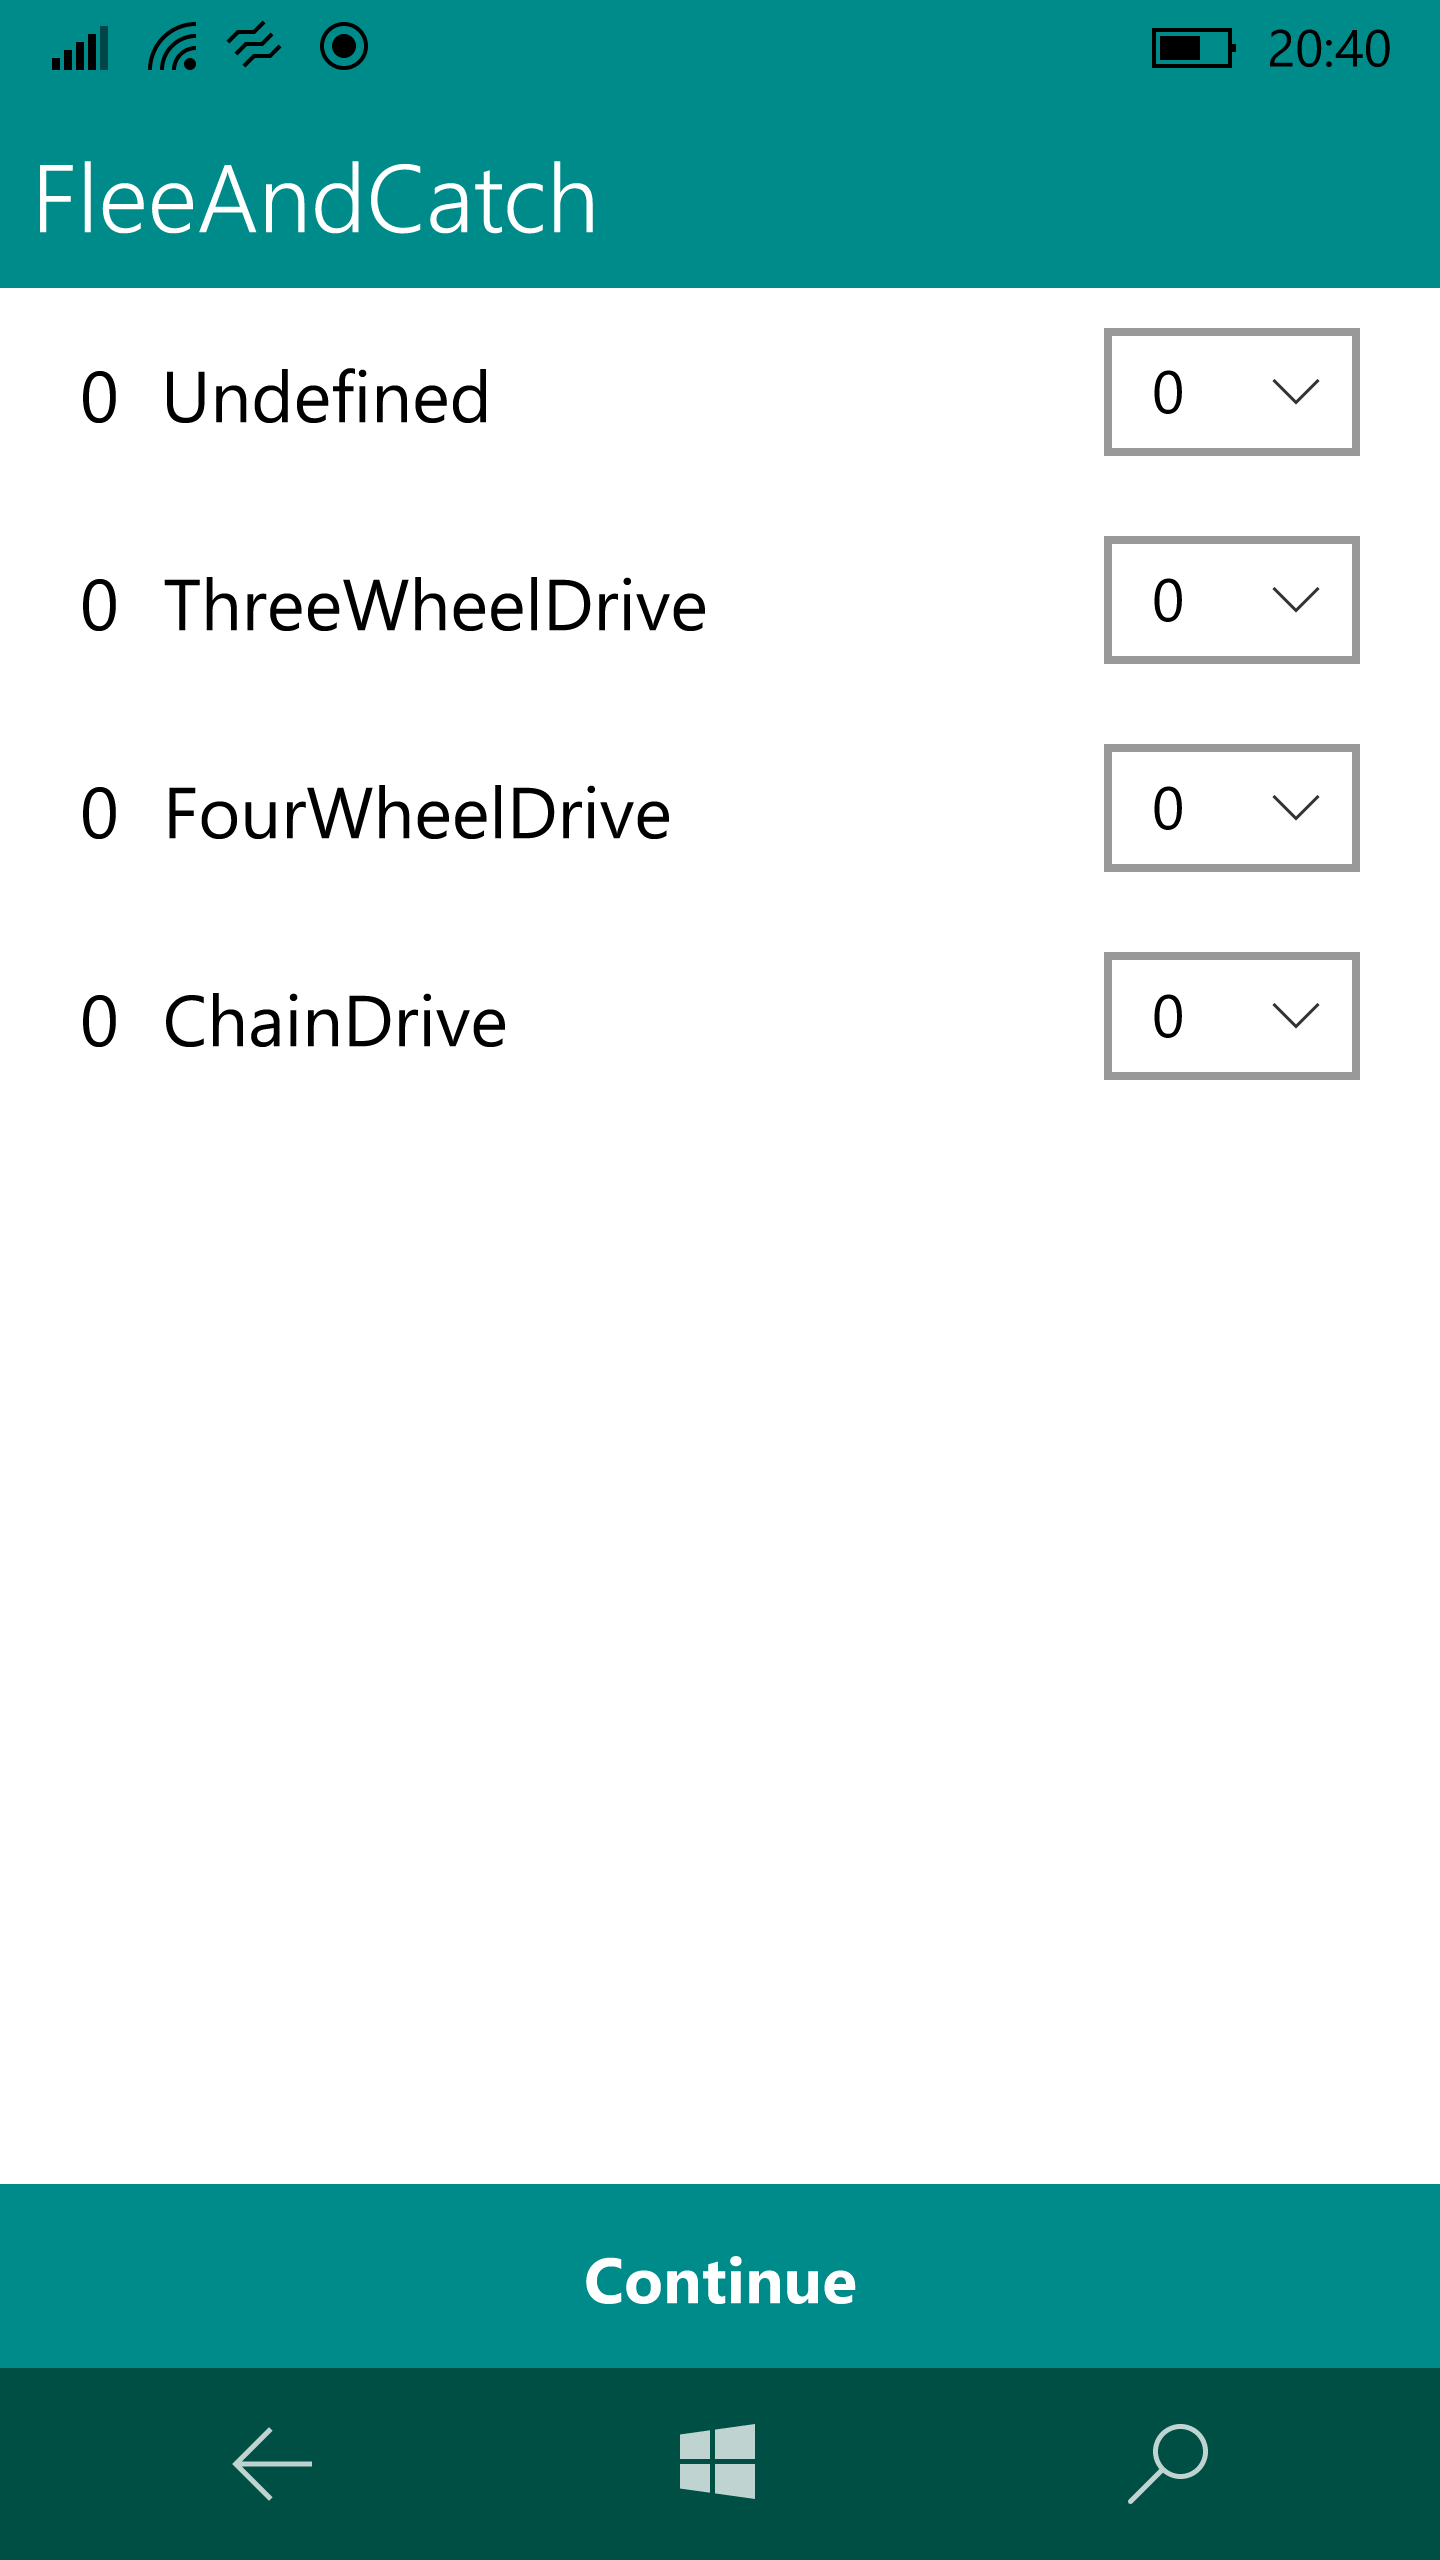
\includegraphics[width=0.4\textwidth]{images/implementation/list.png}
	\end{center}	
	\caption{List Page}
	\label{fig:list}
\end{figure}

\newpage
\paragraph{Szenario Page} stellt die Benutzerschnittselle dar, die einerseits der Steuerung und Überwachung des Schwarmverhaltens dient. Dabei werden laufend die aktuellen Daten der Roboter angezeigt und können durch die Neigungssensoren der eräte gesteuert werden. Diese verhalten sich entsprechend dem ausgewählten SZenario.

\begin{figure}[h]
	\begin{center}
		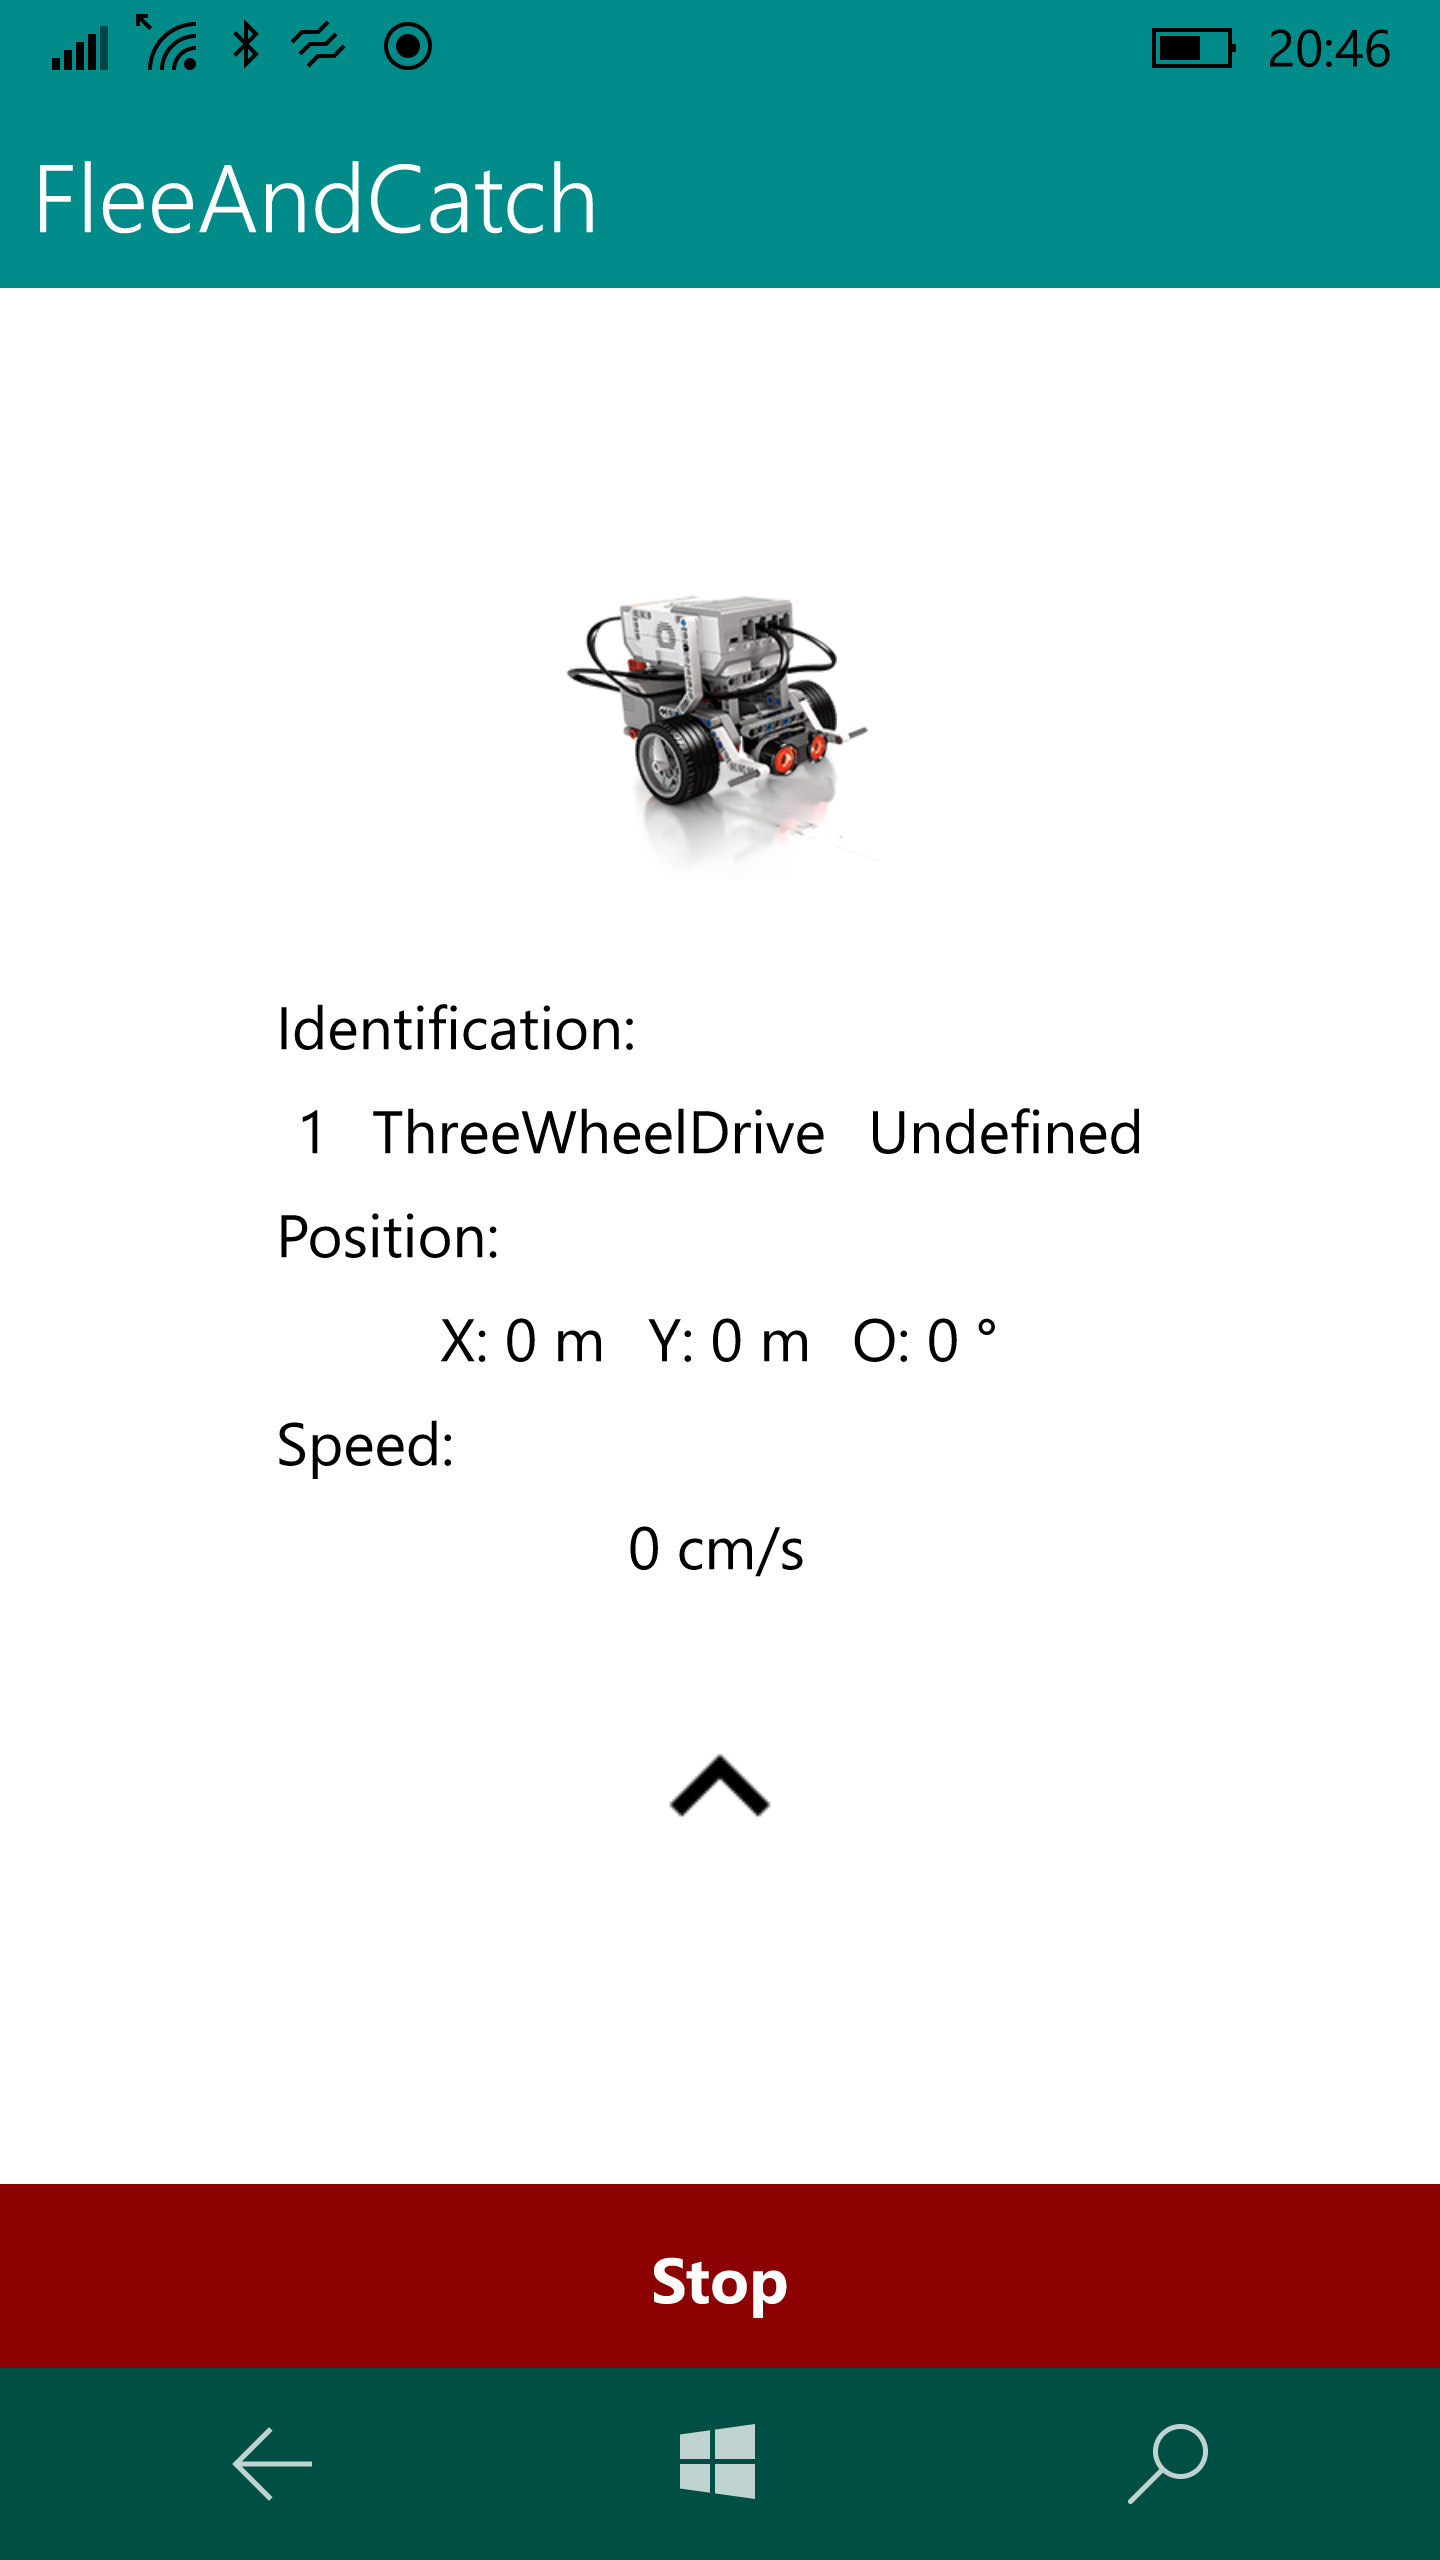
\includegraphics[width=0.4\textwidth]{images/implementation/szenario.png}
	\end{center}	
	\caption{Szenario Page}
	\label{fig:szenario}
\end{figure}

\newpage
\subsubsection{Buisnesslogic} %Logik

\paragraph{Authorization}

\paragraph{Create Szenario}

\paragraph{Szenario}

\newpage

\subsection{Roboter}
Die Implementierung des Roboters stellt das Kernstück bei der Realisierung dieses Projekts dar. 
\\
\\
Da eine komplett detaillierte Beschreibung des ganzen Quellcodes den Umfang dieser Ausarbeitung bei weitem sprengen würde,
werden in diesem Kapitel die wichtigsten Implementierungskonzepte deren Funktionswiese, sowie deren Komponenten dargestellt. 
Für eine vollständig detaillierte Darstellung wird auf den Quellcode und den darin enthalten Kommentare sowie das zugehörige 
github-Wiki (https://github.com/FleeAndCatch-Dev/FleeAndCatch-Docs/wiki) verwiesen.
\subsubsection{Threads}
Für die Umsetzung der Szenarien ist es erforderlich das der Roboter verschiedene Dinge parallel erledigt. Zum einen muss die 
ständige und zeitnahen Kommunikation mit dem Backend aufrecht erhalten werden, um zum einen Steuerdaten sowie die Positionsdaten
der anderen Roboter für die Bewegungsberechnung zu empfangen. Andererseits müssen über diese Verbindung die eigenen Daten übermittelt
an das Backend übermittelt werden. Darüber hinaus muss die eigentliche Steuerung des Roboters erfolgen. \\
Zur Realisierung all dieser Aufgaben sind innerhalb des Roboters die folgenden X Threads implementiert:
\begin{itemize}
	%   ###############################################################################################################################
	\item{Hauptthread (main thread)}
	%   ###############################################################################################################################
	\item{Kommunikationsthread (connectionThread)}
	%   ###############################################################################################################################
	\item{Steuerungsthread (steeringThread)}
	%   ###############################################################################################################################
	\item{Datenerfassungsthread (synchronizeThread)}
	%   ###############################################################################################################################
\end{itemize}
In den folgenden Abschnitten werden die einzelnen Threads sowie ihre Aufgaben dargestellt:
\paragraph{Hauptthread}
Der Hauptthread ist der Thread welcher beim Programmstart (Aufruf der Funktion public static void main(String[] args)) automatisch 
erzeugt wird und der immer vorhanden ist. Durch diesen Thread werden in der Initialisierungsphase alle anderen Threads die 
zur Kommunikation, Steuerung und Datenerfassung benötigt werden erzeugt. 
\paragraph{Kommunikationsthread}
\paragraph{Steuerungsthread}
Der Steuerungsthread hat wie der Name schon sagt die Aufgabe den Roboter zu steuern das heiß seine Geschwindigkeit und Bewegungsrichtung 
umzusetzen. Implementiert ist der Steuerungsthread in der RobotController Klasse die als Schnittstelle zwischen der Kommunikation und den
Roboterfunktionalitäten fungiert. \\
Die konkrete Umsetzung der Steuerung die durch diesen Thread erfolgt wird im Abschnitt X.X beschrieben.
\paragraph{Datenerfassungsthread}
Neben dem Empfangen von Daten und der Umsetzung der Steuerung muss der Roboter auch seine eigen Daten wie Position, Orientierung und 
Geschwindigkeit kontinuierlich erfassen und an das Backend übermitteln so das diese Informationen den anderen Robotern zur Verfügung
gestellt werden können. Da dieser Thread dazu auf Funktionalitäten des Roboters zugreift ist auch dieser innerhalb der RoboterController
Klasse implementiert.
\\
Die Realisierung der Datenerfassung ist weit weniger komplex als die der Steuerung des Roboters. 
Die Abbildung X.X zeigt das Zusammenspiel der einzelnen Threads bzw. den Ablauf ihrer Erzeugung und Terminierung:
\subsubsection{Klassen}
Neben den verschiedenen Threads enthält das Roboterprogramm zahlreiche Klassen durch welche die vielfältigen Funktionen abgebildet 
werden die, der Roboter zur Realisierung der verschiedenen Szenarien mitbringen muss. 
\paragraph{Klassenstruktur}
\color{finishing}             % Farbe die angibt welchen Status der folgende Abschnitt hat!
% Eigentlicher Text:
Zur Strukturierung und einer sauberen Trennung der einzelnen Klassen und ihren Sichtbarkeiten, sind diese in verschiedenen 
Paketen (Java-Packages) organisiert. Diese Klassenstruktur ist hierarchisch aufgebaut, orientiert sich an den grundlegenden 
Bestandteilen des Programms (Kommunikation, Roboterkontrolle etc.) und granuliert in einzelnen Unterpakete anhand der Objekten 
welche die jeweiligen Klassen darstellen bzw. welche Funktionen diese bieten. \\
Bei der Umsetzung wurden die Klassen in den folgenden vier großen Paketbereiche strukturiert.
\begin{itemize}
	%   ###############################################################################################################################
	\item{Kommunikation (\code{flee\_and\_catch.robot.communication})} -- Enthält sämtliche Klassen die für die Kommunikation mit dem
	Backend notwendig sind dazu zählen die Eigentlichen Kommunikator (Sockets), die verschieden Kommandos sowie serialisierbare 
	Datenobjekte.
	%   ###############################################################################################################################
	\item{Roboter (\code{flee\_and\_catch.robot.robot})} -- Hier befinden sich alle Klassen die direkten Zugriff bzw. Einfluss auf den 
	physischen Roboter haben. Dies sind hauptsächlich Sensoren, das Roboter-Interface, Klassen die einen konkreten Roboter darstellen, 
	sowie die zentrale Steuerklasse >>RoboterController<<.
	%   ###############################################################################################################################
	\item{View (\code{flee\_and\_catch.robot.view})} -- Enthält Klassen die der Anzeige d.h Ansteuerung des LCD-Displays des
	Roboters dienen. Zwar ist das LCD-Display auch Bestandteil des Roboters, es wurde sich aber für eine Trennung dieser beiden 
	Bereiche entschieden da diese möglichst unabhängig voneinander bleiben sollten.
	%   ###############################################################################################################################
	\item{Konfiguration (\code{flee\_and\_catch.robot.configuration})} -- Zentrales Paket welches Klassen zur Konfiguration 
	der verschiedenen Programmteile enthält.
	%   ###############################################################################################################################
\end{itemize}
Innerhalb dieser Hauptpakete existieren zahlreiche weitere Unterpakete welche die Klassen weiter strukturieren. Die saubere Einordnung
und Trennung der Programmklassen ermöglicht es in Verbindung mit der Festlegung entsprechender Sichtbarkeiten, die Klassen gegeneinander 
abzuschotten. So wird erreicht, dass die Programmteile lediglich über die vorgesehenen Schnittstellen miteinander interagieren und die
einzelnen Klassen nur diejenigen sehen und ansprechen können die sie tatsächlich benötigen. Zudem hilft es dem Programmierer bei der Orientierung und dem Programmverständnis.
\medskip
\newline
In den nächsten Abschnitten werden die wichtigsten Klassen und Interfaces des Programms näher beschrieben und ihre Rolle bei der 
Realisierung des durch die Roboter abgebildeten Schwarmverhaltens erläutern.
\paragraph{Das Roboter Interface}
\color{process}             % Farbe die angibt welchen Status der folgende Abschnitt hat!
% Eigentlicher Text:
Das Roboter Interface dient als Implementierungsvorlage für Klassen die einen Roboter in seiner jeweiligen physischen Gestalt d.h. mit
der jeweiligen Antriebsform, seinen verbauten Sensoren etc darstellen. Innerhalb dieses Interfaces sind sämtliche Funktionalitäten 
und Methoden definiert, die ein konkreter Roboter bzw. die entsprechende Klasse, die diesen repräsentiert implementieren muss um durch 
das Programm gesteuert und in die entsprechenden Szenarien integriert werden zu können. \\
Innerhalb dieses Interface werden dazu verschiedene Methoden zur Steuerung sowie Abfrage von Roboterparametern definiert. Die durch 
diese Methoden dargestellten Funktionalitäten sind von so grundlegender Natur das diese durch jeden Roboter realisiert bzw. umgesetzt 
werden können, wenn auch abhängig von seiner Bauart auf andere Weise. \\
Folgende Auflistung gibt einen Überblick über die wichtigsten diese Methoden und erläutert kurz die durch sie zur realisierende Funktion.
\begin{itemize}
	%   ###############################################################################################################################
	\item{\code{void forward()}} -- Soll den Roboter geradeaus vorwärts fahren lassen.
	%   ###############################################################################################################################
	\item{\code{void backward()}} -- Soll den Roboter geradeaus rückwärts fahren lassen.
	%   ###############################################################################################################################
	\item{\code{void backward()}} -- Soll den Roboter sich nach rechts oder linkes bewegen lassen abhängig von der übergebenen Richtung
	(Direction-Objekt).
	%   ###############################################################################################################################
	\item{\code{void stop()}} -- Soll den Roboter anhalten.
	%   ###############################################################################################################################
	\item{\code{void increaseSpeed()}} -- Soll die Geschwindigkeit des Roboters erhöhen (Iterativ bei jedem Aufruf).
	%   ###############################################################################################################################
	\item{\code{void increaseSpeed()}} -- Soll die Geschwindigkeit des Roboters verringern (Iterativ bei jedem Aufruf).
	%   ###############################################################################################################################
	\item{\code{boolean isMoving()}} -- Soll true zurückgeben wenn sich der Roboter bewegt.
	%   ###############################################################################################################################
	\item{\code{Position getPosition()}} -- Soll die aktuelle Position und Orientierung des Roboters in einem speziellen 
	Position-Objekt zurückgeben.
	%   ###############################################################################################################################
	\item{\code{float getRealSpeed()}} -- Soll tatsächliche (nicht eingestellte) Geschwindigkeit des Roboters zurückgeben.
	%   ###############################################################################################################################
	\item{\code{Robot getJSONRobot()}} -- Soll alle wichtigen Roboterdaten einem speziellen Roboter-Objekt zurückgeben welches 
	serialisierbar ist und damit via JSON-Objekt an des Backend übertragen werden kann.
	%   ###############################################################################################################################
\end{itemize}
Durch die Vorgaben und Verwendung dieser grundlegenden und universellen Funktionalitäten für die Programm-, Szenarien- und Steuerlogik 
ist es mögliche eine generische und flexible Implementierung zu schaffen. Da ein Roboter immer als Objekt dieses Interfaces betrachtet 
und angesprochen wird ist das restliche Programm vollkommen unabhängig von der konkreten Ausprägung des jeweilige Roboter und kennt 
diese nicht mal. Es beschränkt sich bei der Interaktion mit dem Roboter auf die in diesem Interface definierten Methoden. \\
Der Vorteil dieser Implementierung liegt darin, dass durch dieses generische Programmierung lediglich eine neuen Klasse die dieses 
Interface implementiert notwendig ist um einen neue Art von Roboter zu Realisierung und in das Projekt mit sämtlichen Szenarien zu 
integrieren. Dadurch ist das Programm leicht erweiterbar und es steigert seine Wiederverwendbarkeit. \\
Wie diese konkrete Implementierung der durch diese Methoden definierten Funktionen zu realisieren ist hängt natürlich vom jeweilige
Roboter und seinem Aufbau ab und muss durch den Programmiere entsprechend umgesetzt werden.
\paragraph{Die ThreeWheelDrive Klasse (Eine konkrete Roboter Klasse)}
\color{process}             % Farbe die angibt welchen Status der folgende Abschnitt hat!
% Eigentlicher Text:
Die Klasse >>ThreeWheelDrive<< repräsentiert den \glqq{}Standard\grqq{}-Roboter im Projekt. Sie bildet den in Abbildung X.X zu 
sehenden Roboter mit seine relevanten Komponenten wie Sensoren, Motoren sowie relevanten geometrischen und physischen Parametern ab.
Die Klasse implementiert das Roboter-Interface mit den dort definierten Methoden. 
\paragraph{Die RoboterController Klasse}
Die >>RobotController<<-Klasse übernimmt eine zentrale Rolle bei der Umsetzung der Roboter-Steuerung. Die Klasse stellt die Schnittstelle
zum physischen Roboter dar. Sämtliche Steuerkommandos und Sensorabfragen werden über diese Klasse realisiert. Durch diese einheitliche 
Schnittstelle wird es möglich die Steuerung und ... unabhängig von dem konkreten vorhandenen Roboter (Dreirädriger, Vierrädriger etc)
zu realisieren. Dazu nutzt der RoboterController intern eine Instanz des "Roboter" Interfaces was eine Ansteuerung des Roboters 
\\
Die folgende Abbildung zeigt die der verschiedenen Komponenten:
\subsubsection{Steuerung}
Eine der Hauptaufgaben des Roboterprogramms ist die Steuerung des Roboters. Dabei muss das Programm die folgende zwei 
grundlegenden Steuerungsarten unterscheiden und realisieren.
\begin{itemize}
	%   ###############################################################################################################################
	\item{Direkte Steuerung} -- Bei der direkten Steuerung erhält das Programm über das Backend von der App direkte Steuerbefehle wie
	Rechts, Links, Schneller, Langsamer welche das Programm dann in die entsprechende Bewegung des Roboters umsetzen muss.
	%   ###############################################################################################################################
	\item{Indirekte Steuerung} -- Bei der indirekten Steuerung bekommt das Programm keinen konkreten Steuerbefehle sondern muss basierend
	auf den Positionsdaten der anderen Roboter und dem vorherrschenden Szenario die notwendigen Steuerbefehle des Roboters berechnen.
	%   ###############################################################################################################################
\end{itemize}
Dabei erfolgt das Empfangen und Verarbeiten der jeweiligen Daten jeweils zyklisch in einem konfigurierbaren Zeitintervall. Beide Steuerungsarten
basieren auf dem grundlegenden Prinzip das die Daten (Steuerbefehle oder Positionsdaten) durch den X-Thread erfasst und gespeichert werden.
Der Stuerungsthread widerun liest diese Daten aus und führt die entsprechenden Roboterbefehle aus.
\paragraph{Allgemein}
\paragraph{Realisierung beim ThreeWheelDrive}
\subsubsection{Datenerfassung}
\subsection{Backend}
Das Backend ist die Kommunikations- und Verwaltungszentrale des Projekts und bildet das Rückgrat der Kommunikation. Es verwaltet die 
Devices im Kontext der einzelnen Szenarien und sorgt für den Datenaustausch zwischen den verschieden Geräten. \\
Realisiert ist des Backend wie auch der Roboter in der Programmiersprache Java. Das bringt neben der plattformunabhängigen 
Lauffähigkeit des Programms noch weitere Vorteile mit sich. So können vor allem Programmkomponenten welche die Kommunikation und
den Datenaustausch betreffen für die Roboter- bzw. Backend-Implementierung wiederverwendet werden und müssen nicht komplett neu
implementiert werden.
Im Folgenden werden die zentralen Komponenten des Backends vorgestellt.
\subsection{Aufbau}
\subsubsection{Server}
Zur Realisierung der Kommunikation verfügt das Backendprogramm über eine Klasse namens Server. Innerhalb dieser Klasse ist ein
Server-Socket implementiert welches den Endpunkt einer TCP-Verbindung darstellt Abschnitt siehe X.X. Dieses Server-Socket wird
nach dem Programmstart durch aufrufe der Methode \code{open()} mit IP-Adresse und Port initialisiert und kann anschließend 
darüber Nachrichten (z.B. Aufbauanfragen für eine TCP-Verbindung) entgegennehmen. \\
Die Abbildung X zeigt die Funktion \code{open()} welche eine Server-Socket initialisiert und den listenerThread startet.
\begin{figure}[ht]
	\centering
	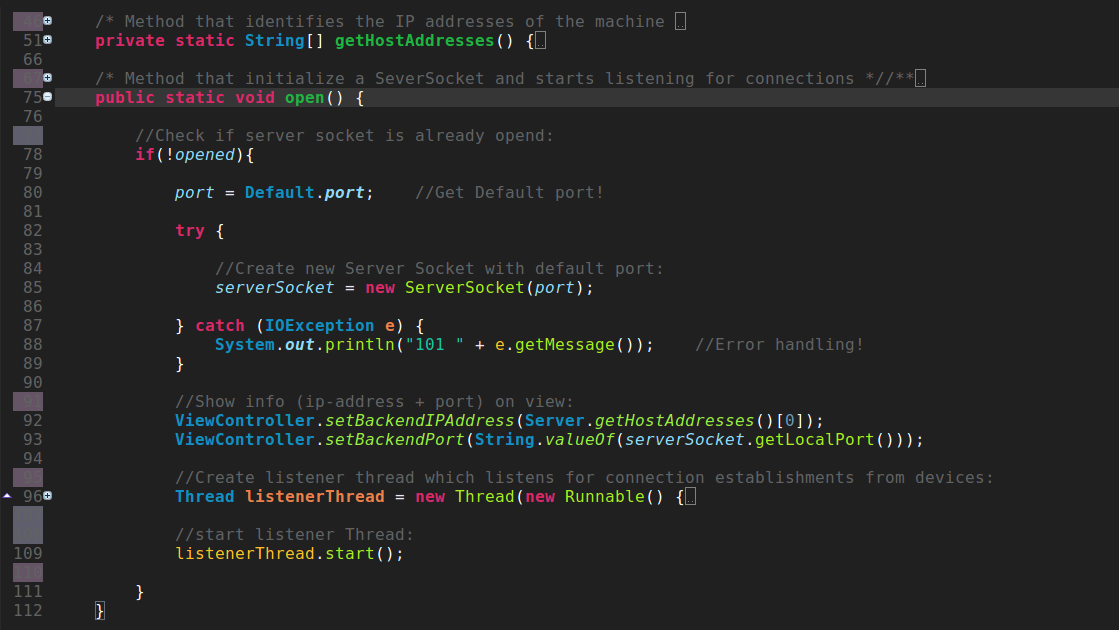
\includegraphics[width=1.0\textwidth]{images/implementation/SeverOpenMethod.png}
	\caption[\code{open()}-Methode der Sever-Klasse im Backend]{\code{open()}-Methode der Sever-Klasse im Backend}
	\label{fig:ev3system}
\end{figure}
Nach der Initialisierung des Server-Socket wird ein Thread gestartet (listenerThread), welcher zyklisch die Methode \code{listen()}
aufruft. Die Aufgabe dieses Threads ist es kontinuierlich auf Verbindungsaufbauwünsche durch Roboter oder Apps zur warten und bei
deren eintreffen diese zu verarbeiten. \\
Die Abbildung X zeigt die Methode \code{listen()} in der ankommende Verbindungsaufbauwünsche verarbeitet werden.
\begin{figure}[ht]
	\centering
	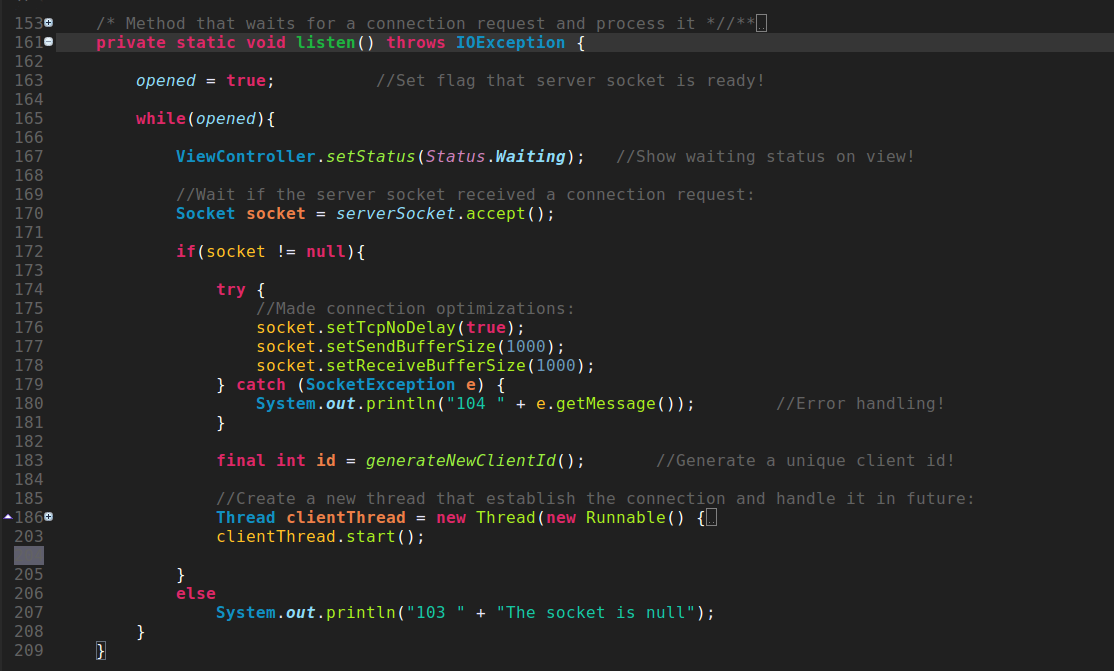
\includegraphics[width=1.0\textwidth]{images/implementation/SeverListenMethod.png}
	\caption[\code{listen()}-Methode der Sever-Klasse im Backend]{\code{listen()}-Methode der Sever-Klasse im Backend}
	\label{fig:ev3system}
\end{figure}
Trifft ein Verbindungsaufbauwunsch ein wird für diesen, vom Server-Socket ein neues Socket Objekt zurück geliefert welches 
ab sofort eine unabhängige Verbindung zum anfangenden Device repräsentiert und ein Senden von Nachrichten in beide Richtungen 
ermöglicht.\\
Anschließend werden auf diesem Socket-Objekt noch ein paar Optimierungen durchgeführt um die Latenz der Kommunikation mit dem
Device möglichst gering zu halten. Dazu wird zum einen der Nagle-Algorithmus deaktiviert, siehe Abschnitt X sowie entsprechende
Puffergrößen festgelegt. \\
Danach wird ein Thread erzeugt der ab sofort die Kommunikation dieser Verbindung verwaltet. Dazu wird dieser an ein neues Client-Objekt 
gekoppelt, welches das zugehörige Socket-Objekt aufnimmt. Mit der Erzeugung dieses Client-Objekts der Übergabe des Socket-Objekts an diese und
die Zuordnung des entsprechenden Thread zur Verbindungsverarbeitung ist die Verbindung zu einem Device vollständig initialisiert. 
Ab sofort wird das entsprechende Device (App oder Robot) durch das Client-Objekt repräsentiert und kann durch dieses angesprochen werden. Dazu
werden sämtliche Clients in deiner Array-Liste gespeichert und sind durch eine eindeutige ID identifizierbar.
\subsubsection{Client}
Neben der Server Klasse ist die Client Klasse die zentrale Komponente zum Empfangen und Senden von Daten an die einzelnen Devices.
Während die Server-Klasse auf Verbindungsaufbauwünsche der Geräte die sich am Backend anmelden wollen warten, repräsentieren die Clients
eine Device inklusive einer vollwertige TCP-Verbindung.  
\subsubsection{Interpreter}
Die Interpreter Klasse ist zuständig für die Interpretation der am Backend eintreffenden Datenpakete der verschiedenen Devices. Dazu enthält
jedes Client-Objekt eine eigene Instanz der Klasse Interpreter, so dass eine parallele Verarbeitung ohne Beeinflussungen oder Wartezeiten 
möglich ist. \\
Die Interpretation der Datenpakete besteht aus zwei grundlegenden Schritte:
\begin{enumerate}
	%   ###############################################################################################################################
	\item{Parsen des als String vorliegenden Datenpakets in ein JSON-Objekt}
	%   ###############################################################################################################################
	\item{Weiterverarbeitung des JSON-Objekts anhand des vorliegenden Kommandotyps}
	%   ###############################################################################################################################
\end{enumerate}
Den ersten Schritt realisiert die Methode \code{public void parse(String pCommand)}. Zur Umwandlung des vorliegenden Strings verwendet
die Methode dazu eine Funktionalität der Bibliothek >>org.json<<. Anschließend wird das geparste JSON-Object abhängige von seinem
Kommandotyp durch eine entsprechende Methode weiterverarbeitet. \\
Die Abbildung X zeigt den Quellcode des Parse-Vorgangs in der Methode Vorgangs \code{public void parse(String pCommand)}.
\begin{figure}[ht]
	\centering
	\includegraphics[width=1.0\textwidth]{images/implementation/InterpreterParseMethod.png}
	\caption[Ausschnitt der \code{parse()}-Methode der Interpreter-Klasse im Backend]{Ausschnitt der \code{parse()}-Methode der Interpreter-Klasse im Backend}
	\label{fig:ev3system}
\end{figure}
\newline
Die folgende Auflistung zeigt die Methoden der Interpreter Klasse:
\begin{itemize}
	%   ###############################################################################################################################
	\item{\code{public void parse(String pCommand)}} -- Diese Methode führt den eigentlichen Parse-Vorgang durch um das als String
	vorliegende Datenpaket (pCommand) in ein JSON-Objekt zu konvertieren.
	%   ###############################################################################################################################
	\item{\code{private void connection(JSONObject pCommand)}} -- Verarbeitet ein als JSON-Objekt vorliegendes Datenpaket vom Typ 
	Kommandotyp Connection.
	%   ###############################################################################################################################
	\item{\code{private void synchronization(JSONObject pCommand)}} -- Verarbeitet ein als JSON-Objekt vorliegendes Datenpaket vom 
	Typ Kommandotyp Synchronization.
	%   ###############################################################################################################################
	\item{\code{private void szenario(JSONObject pCommand)}} -- Verarbeitet ein als JSON-Objekt vorliegendes Datenpaket vom Typ 
	Kommandotyp Szenario. Dazu existieren folgenden folgende Methoden die die Daten abhängig vom vorliegenden Szenario verarbeiten:
	\begin{itemize}
			%   ###############################################################################################################################
			\item{\code{private void szenarioControl(SzenarioCommand pCommand)}}
			%   ###############################################################################################################################
			\item{\code{private void szenarioSynchron(SzenarioCommand pCommand)}}
			%   ###############################################################################################################################
			\item{\code{private void szenarioFollow(SzenarioCommand pCommand)}}
			%   ###############################################################################################################################
	\end{itemize}
	%   ###############################################################################################################################
	\item{\code{private void exception(JSONObject pCommand)}} -- Verarbeitet ein als JSON-Objekt vorliegendes Datenpaket vom Typ 
	Kommandotyp Exception.
	%   ###############################################################################################################################
\end{itemize}
Aus der Auflistung ist gut ersichtlich das es für jeden Kommandotyp eine eigene Methode zu dessen Verarbeitung implementiert wurde.
Da diese immer nach dem selben Prinzip die Datenverarbeitung vornehmen wird im folgenden exemplarisch auf eine dieser Methode 
eingegangen um dieses Prinzip zu verdeutlichen. \\

\subsubsection{Device \& Szenario Controller}
Neben den für die Kommunikation wichtigen Komponenten spielen bei der Realisierung des Backends auch die Controller-Klassen eine 
zentrale Rolle, da diese wichtige Verwaltungsfunktionen bereit stellen. Sie sind für die Verwaltung der verschiedenen Devices 
und Szenarien zuständig. \\
Dazu existieren die folgenden Controller-Klassen:
\begin{itemize}
	%   ###############################################################################################################################
	\item{AppController} -- Der AppContoller verwaltet alle am Backend angemeldeten Apps.
	%   ###############################################################################################################################
	\item{RobotContoller} -- Der RoboterContoller verwaltet alle am Backend angemeldeten Roboter.
	%   ###############################################################################################################################
	\item{ScenarioController} -- Der AppContoller verwaltet sämtliche aktiven Szenarien.
	%   ###############################################################################################################################
\end{itemize}
Die beiden Klassen AppController und RoboterController bestehen im wesentlichen aus einer ArrayList, in welcher sämtliche Apps bzw. 
Roboter die am Backend angemeldet sind gespeichert werden. Dazu werden die Devices durch Objekte entsprechender Klassen in der 
ArrayList repräsentiert. 

Alle drei Klassen arbeiten mit statischen Datenstrukturen und Methoden da sie ...
\subsubsection{Die GUI}
Neben den rein Funktionalen Komponenten des Backends verfügt dieses auch über eine grafische Benutzeroberfläche die Informationen zu
den angemeldeten Geräten und den existierenden Szenarien zur Verfügung stellt. Diese Benutzeroberfläche ist so realisiert das diese 
komplett losgelöst von den der eigentlichen Funktionalität des Backend ist. Sie setzt lediglich auf dem eigentlichen Programm auf und
ist zu dessen Ausführung nicht notwendig. Dadurch ist es möglich das Programm komplett ohne grafische Benutzeroberfläche zu starten so
das es im Hintergrund laufen kann und lediglich als Verwaltungs- und Kommunikationsservice dient. Ob die grafische Benutzeroberfläche  
aktiviert ist oder nicht wird beim Programmstart durch entsprechenden Parametern festgelegt. \\
Der Nutzen der GUI bestand für uns hauptsächlich im Monitoring und bei der Identifikation sowie dem Aufspüren von Fehlern während der 
Entwicklung. \\
Realisiert ist die grafische Benutzeroberfläche mit dem JavaFX-Framework welches Bestandteil der Java-Bibliothek ist uns somit wie 
Java ebenfalls plattformunabhängig lauffähig ist. Zu ihrer Ansteuerung dient eine spezielle Klasse namens
>>ViewController<< welche lediglich Informationen des eigentliche Programms entgegen nimmt und an die eigentliche Benutzeroberfläche 
(View) weiterreicht sofern diese aktiviert wurde. Umgekehrt werden jedoch keine Benutzereingaben von der GUI an das Programm 
weitergereicht, sondern dienen lediglich zur Manipulation der Anzeige so das dieses komplett unabhängig ist. Lediglich das Beenden 
das kompletten Programms ist über die grafische Benutzeroberfläche möglich.
Abbildung X.X zeigt einen Screenshot der grafischen Benutzeroberfläche des Backends. \\
\\
Da die grafische Benutzeroberfläche jedoch nicht zur eigentlichen Funktionalität des Backends beiträgt soll an dieser Stelle nicht 
weiter eingegangen werden.
\begin{comment}
Aufbau
Interpreter
Mechanismen
GUI
\end{comment}


\begin{comment}
Aufbau
Robot
RobotController
EV3 Library
GUI
\end{comment}
	\section{Evaluation}
	\section{Zusammenfassung und Ausblick}
	\bibliography{literatur}
	\section*{Anhang}

\includepdf[pages={1-1}]{pdf/Anmeldung_Studienarbeit_Simon_Lang}

	
\end{document}